\documentclass[twoside,a4paper]{book}
\usepackage{geometry}
\usepackage{booktabs}
\usepackage{dirtytalk} % for \say command


%\usepackage[english]{babel}
\usepackage[english]{babel}
\usepackage[T1]{fontenc}
\usepackage{graphicx}

\usepackage{float}
\floatstyle{ruled}
\newfloat{program}{thp}{lop}
\floatname{program}{Program}

% Pakete für Mathe:
\usepackage{amsfonts,amsmath,amsthm,amscd,amssymb,array}
\usepackage{nicefrac}

\usepackage{xcolor, fancybox}
\usepackage{fix-cm}
\usepackage{lmodern}

\definecolor{6gtandempurple}{HTML}{DD8A2E}
\usepackage[colorlinks=true, linkcolor=6gtandempurple, anchorcolor=6gtandempurple, citecolor=6gtandempurple, filecolor=6gtandempurple, urlcolor=6gtandempurple]{hyperref} % Use the color defined 

% Pakete für Algorithmen
%\usepackage{algorithm,ifthen,url,algpseudocode}
\usepackage{algpseudocode,algorithm}

%Pakete zum Erstellen von ps-Grafiken
\usepackage{pstricks,pst-plot,pst-node}

% Paket, mit dem man festlegen kann, was geschehen soll, wenn die Seite voll ist.
\usepackage{afterpage}


\usepackage{marvosym}

% "Einrichten" des theorem-Paketes:
\newtheorem{thm}{Satz}[chapter]
\newtheorem{lem}[thm]{Lemma}
\newtheorem{cor}[thm]{Corollary}
\newtheorem*{nnlem}{Lemma}
\newtheorem*{nnthm}{Theorem}

\theoremstyle{definition}
\newtheorem{exmp}[thm]{Example}
\newtheorem*{nnexmp}{Example}
\newtheorem{defn}[thm]{Definition}
\newtheorem*{nndefn}{Definition}

\theoremstyle{remark}
\newtheorem{rem}[thm]{Remark}
\newtheorem*{nnrem}{Remark}

% Einige Makros:
\newcommand{\modulo}{\mbox{mod }}
\newcommand{\Z}{\mathbb{Z}}
\newcommand{\N}{\mathbb{N}}
\newcommand{\J}{\mathbb{J}}
\newcommand{\HD}{\mathbb{P}}
\newcommand{\D}{\mathbb{D}}
\newcommand{\R}{\mathbb{R}}
\newcommand{\CO}{\mathcal{O}}
\newcommand{\F}{\mathbb{F}}
\newcommand{\divisor}{\mathrm{div}}
\newcommand{\ord}{\mathrm{ord}}
\newcommand{\supp}{\mathrm{supp}}
\newcommand{\ggt}{\mathrm{ggt}}
\newcommand{\charac}{\mathrm{char}}
\renewcommand{\algorithmicrequire}{\textbf{Input:}}
\renewcommand{\algorithmicensure}{\textbf{Output:}}
%\renewcommand{\listalgorithmname}{Algorithms}
\makeatletter
\renewcommand{\ALG@name}{Algorithm}

\newcommand{\option}{{\small -}{\small -}}
\newenvironment{bew}{\begin{proof}[Proof]}{\end{proof}}
% Komfortabler Sachen in den Index aufnehmen:
\newcommand{\idx}[1]{#1\index{#1}}

\newcommand{\bl}{\color{blue}}
\newcommand{\bk}{\color{black}}
\newcommand{\rd}{\color{red}}
\newcommand{\gr}{\color{green}}

% Now defining header and footer
%\usepackage{scrpage2} % for some decent header-lines
%\clearscrheadfoot % clear style
%\lehead{\pagemark} % page left even
%\lohead{\headmark} % heading left odd
%\rohead{\pagemark} % page right odd
%\rehead{\headmark} % heading right even
%\setheadsepline{.5pt} % thickness of separating line
%\setfootsepline{.5pt} % thickness of separating line
%\lefoot{
\includegraphics[height=9pt]{ti_veclogo}} % ti left even
%\rofoot{
\includegraphics[height=9pt]{RWTHAACHEN_sw}} % rwth right odd

% Seitenformatierung
% \usepackage[a4paper, top=2.0cm, bottom=1.5cm, hmargin=2.5cm, includehead, includefoot, headheight=15pt]{geometry} % Flexible and complete interface to document dimensions.
\setlength{\parindent}{0cm} % Default space between columns of tabulars
\setlength{\parskip}{5pt plus 2pt minus 1pt}
\clubpenalty = 10000 % Avoid "`Schusterjungen"'
\widowpenalty = 10000 % Avoid "`Waisenkinder"'
\displaywidowpenalty = 10000 %
\tolerance 1000 % Tolerance in linebreaks
\hbadness 1000 % Number at which badness ist reported
\emergencystretch 1.5em 

\usepackage{multirow}

\makeatletter
\DeclareRobustCommand{\Cpp}
{\valign{\vfil\hbox{##}\vfil\cr
   \textsf{C\kern-.1em}\cr
   $\hbox{\fontsize{\sf@size}{0}\textbf{+\kern-0.05em+}}$\cr}%
}
\makeatother
\makeatletter
\DeclareRobustCommand{\ITpp}
{\valign{\vfil\hbox{##}\vfil\cr
   \textsf{IT\kern-.1em}\cr
   $\hbox{\fontsize{\sf@size}{0}\textbf{+\kern-0.05em+}}$\cr}%
}
\makeatother


\makeatletter
\def\blfootnote{\gdef\@thefnmark{}\@footnotetext}
\makeatother

\usepackage[outdir=./figs/]{epstopdf}

\usepackage[capitalise]{cleveref} 

\usepackage[per-mode=symbol]{siunitx}  %usage \SI{35}{\meter\squared}
\DeclareSIUnit{\dBm}{dBm}	% add SI unit "dBm"

\usepackage{cmbright}

% \newcommand{\Cpp}{C\texttt{++}}

\usepackage{caption}
\usepackage{subcaption}

\usepackage{tikz}
\usetikzlibrary{shapes}

\usepackage{siunitx} % Provides the \SI{}{} and \si{} command for typesetting SI units
\usepackage{graphicx} % Required for the inclusion of images
\graphicspath{{./figs/}}
\usepackage[backend=biber,style=ieee]{biblatex}
%\usepackage[backend=biber,language=dutch]{biblatex}
\addbibresource{bib.bib}
\AtBeginBibliography{\footnotesize}
\usepackage{amsmath} % Required for some math elements
\usepackage{lastpage} % know last page (used in fancy header)
\usepackage{fancyhdr} % Fancy Header
\usepackage[xindy, toc, numberedsection, acronym]{glossaries} % glossaries with xindy (recommended) for the indexing phase and show glossaries in TOC, and numberedsection to get a Setion number in the title
\usepackage{url} %The command is intended for email addresses, hypertext links, directories/paths, etc., which normally have no spaces, so by default the package ignores spaces in its argument.
\usepackage{minted} % it allows formatting and highlighting source code
% in addition, Pygments must be installed
% How to install on Windows:
% 1) install python (and add it to your PATH)
% 2) install pip (https://pip.pypa.io/en/stable/installing/)
% 3) install pygments (pip install Pygments)
% add pygments to your PATH, the command "pip show Pygments" shows where the lib is installed
% Of course, pdfLaTeX (or whatever engine/format you use) still has to be called with the -shell-escape option.



\loadglsentries{abbr.tex}
\makeglossaries % generate the glossary
% Any links in resulting glossary will not be "clickable" unless you load the glossaries package after the hyperref package.

\setlength\parindent{0pt} % Removes all indentation from paragraphs

%\renewcommand{\labelenumi}{\alph{enumi}.} % Make numbering in the enumerate environment by letter rather than number (e.g. section 6)

\renewcommand{\arraystretch}{1.2} % Increasing the array stretch factor using \renewcommand{\arraystretch}{<factor>} where <factor> is a numeric value


%----------------------------------------------------------------------------------------
%	DOCUMENT INFORMATION
%----------------------------------------------------------------------------------------
\newcommand{\maintitle}{OFDM with SDR}
\newcommand{\course}{Wireless Communication}
\newcommand{\coursenumber}{B-KUL-JLI1CG}
\newcommand{\class}{4ELICT}

%%%%%%%%%%%%%%%%%%%%%%%%%%%%%% HEADER %%%%%%%%%%%%%%%%%%%%%%%%%%%%%%
\pagestyle{fancy}
\fancyhf{}
\fancyhead[LE,RO]{\course}
\fancyhead[RE,LO]{\maintitle}
% if working with chapters
% \fancyfoot[CE,CO]{\leftmark}
\fancyfoot[LE,RO]{\thepage\ of \pageref*{LastPage}}
%%%%%%%%%%%%%%%%%%%%%%%%%%%%%% HEADER %%%%%%%%%%%%%%%%%%%%%%%%%%%%%%


%%------------------------------ TITLE PAGE -----------------------------
\title{\maintitle \\ \course \\{\small\ (\coursenumber)}} % Title

\author{Gilles \textsc{Callebaut}} % Author name

\date{\today} % Date for the report

\begin{document}\sloppy 
\maketitle



\restoregeometry%              %% restore the layout
\pagenumbering{arabic}% Arabic page numbers (and reset to 1)

{\hypersetup{hidelinks}
\tableofcontents
}

% \listoflistings%
\clearpage
\printglossary[type=\acronymtype,title={Abbreviations}]
\clearpage

\chapter{Introduction}
\blfootnote{This document is highly insipred by and containts work done by Michael Reyer and RWTH Aachen University. The author was allowed to alter and distribute the content provided by them.}

Current broadband wireless standards are based on \gls{ofdm}, a multi-carrier modulation scheme which provides strong robustness against \gls{isi} by dividing the broadband channel into many orthogonal narrowband subchannels in such a way that attenuation across each subchannel stays flat. Orthogonalization of subchannels is performed with low complexity by using the \gls{fft}, an efficient implementation of \gls{dft}, such that the serial high-rate data stream is converted into multiple parallel low-rate streams, each modulated on a different subcarrier.

Many of the currently used wireless standards are using \gls{ofdm} for the physical layer, e.g., \gls{wlan}, \gls{wimax}, \gls{dab}, \gls{dvb}, \gls{dsl}, \gls{lte}, etc. Beside the existing systems there is active research on future systems enhancing the existing standards to improve system performance. The investigation and assessment of information theoretic concepts for wireless resource management of those new systems in real-world scenarios requires flexible testbeds with a wide range of reconfigurable parameters. This functionality is currently offered in \gls{sdr} technology based on general purpose hardware only.

We designed a modular, \gls{sdr} based and reconfigurable framework which treats the \gls{ofdm} transmission link as a black box. The given framework contains transmitter and receiver nodes that are composed of a host commodity computer and a general purpose \gls{rf} hardware, namely \gls{usrp}. Baseband \gls{ofdm} signal processing at host computers is implemented in the GNU~Radio framework, an open source, free software toolkit for building \glspl{sdr}~\cite{GNUR}.

The control and feedback mechanisms provided by the given framework allow for reconfigurable assignments of predefined transmission parameters at the input and estimation of link quality at the output. High flexibility, provided by a large set of reconfigurable parameters, which are normally static in real systems, enables implementation and assessment of different signal processing and resource allocation algorithms for various classes of system requirements.

During this lab exercises the \gls{sdr} concept will be studied. Insight into the high flexibility in system design offered by \gls{sdr} or comparable systems and corresponding architectural constraints will be gained. Within the framework, high reconfigurability of transmission parameters allows for easy assessment and evaluation of \gls{ofdm} system performance in real wireless channel conditions and for comparison with theoretically derived results.

This script is organized as follows. An introduction to basic \gls{ofdm} system's characteristics is given in Chapter~\ref{sec:basic}. In Section~\ref{sec:discmod}, a corresponding discrete-model is introduced and applied for analytical assessment of the influence of system impairments which are discussed in Section~\ref{sec:sysimp}. A short survey of coherent modulation techniques commonly used in \gls{ofdm} systems and their performance evaluation in \gls{awgn} channels are presented in Section~\ref{sec:cohmod}.
Basic principles, architectural concepts of \gls{sdr} and an introduction to GNU~Radio framework are pictured in~\cref{sec:sdrgnur}. In~\cref{sec:sdr}, system benefits and practical limitations of \gls{sdr} are addressed. Deeper insight into GNU~Radio architecture and an example of wireless channel simulation within a given framework can be gained in Section~\ref{sec:gnur}.
In Chapter~\ref{sec:TIOFDM}, a detailed system description of the SDR framework, which will be used for lab exercises, is given.
Finally, the preparatory and lab exercises are described, and corresponding tasks are depicted in Chapters~\ref{ch:preparation} and~\ref{ch:labs}. 

% Students should show understanding of theoretical background by finalizing the preparation exercise given in Section~\ref{sec:preparation}. In Section~\ref{sec:awgn}, Lab 1 should be conducted where system performance of OFDM system in real wireless channel should be evaluated and compared with theoretical results derived in preparation exercise. Impact of frequency selective channel to system performance should be analyzed in Lab 2, given in Section \label{sec:frsel}.






\chapter{OFDM Basics and Impairments}\label{sec:basic}

In this chapter the basic principles of \gls{ofdm} baseband signal processing are given and an appropriate discrete-time OFDM system model is introduced. In the following section impact and prevention of synchronization errors and equalization are explained. Finally, digital modulations commonly used in wireless transmission standards are described in~\cref{sec:cohmod}.

\begin{figure}[htbp]
\centering
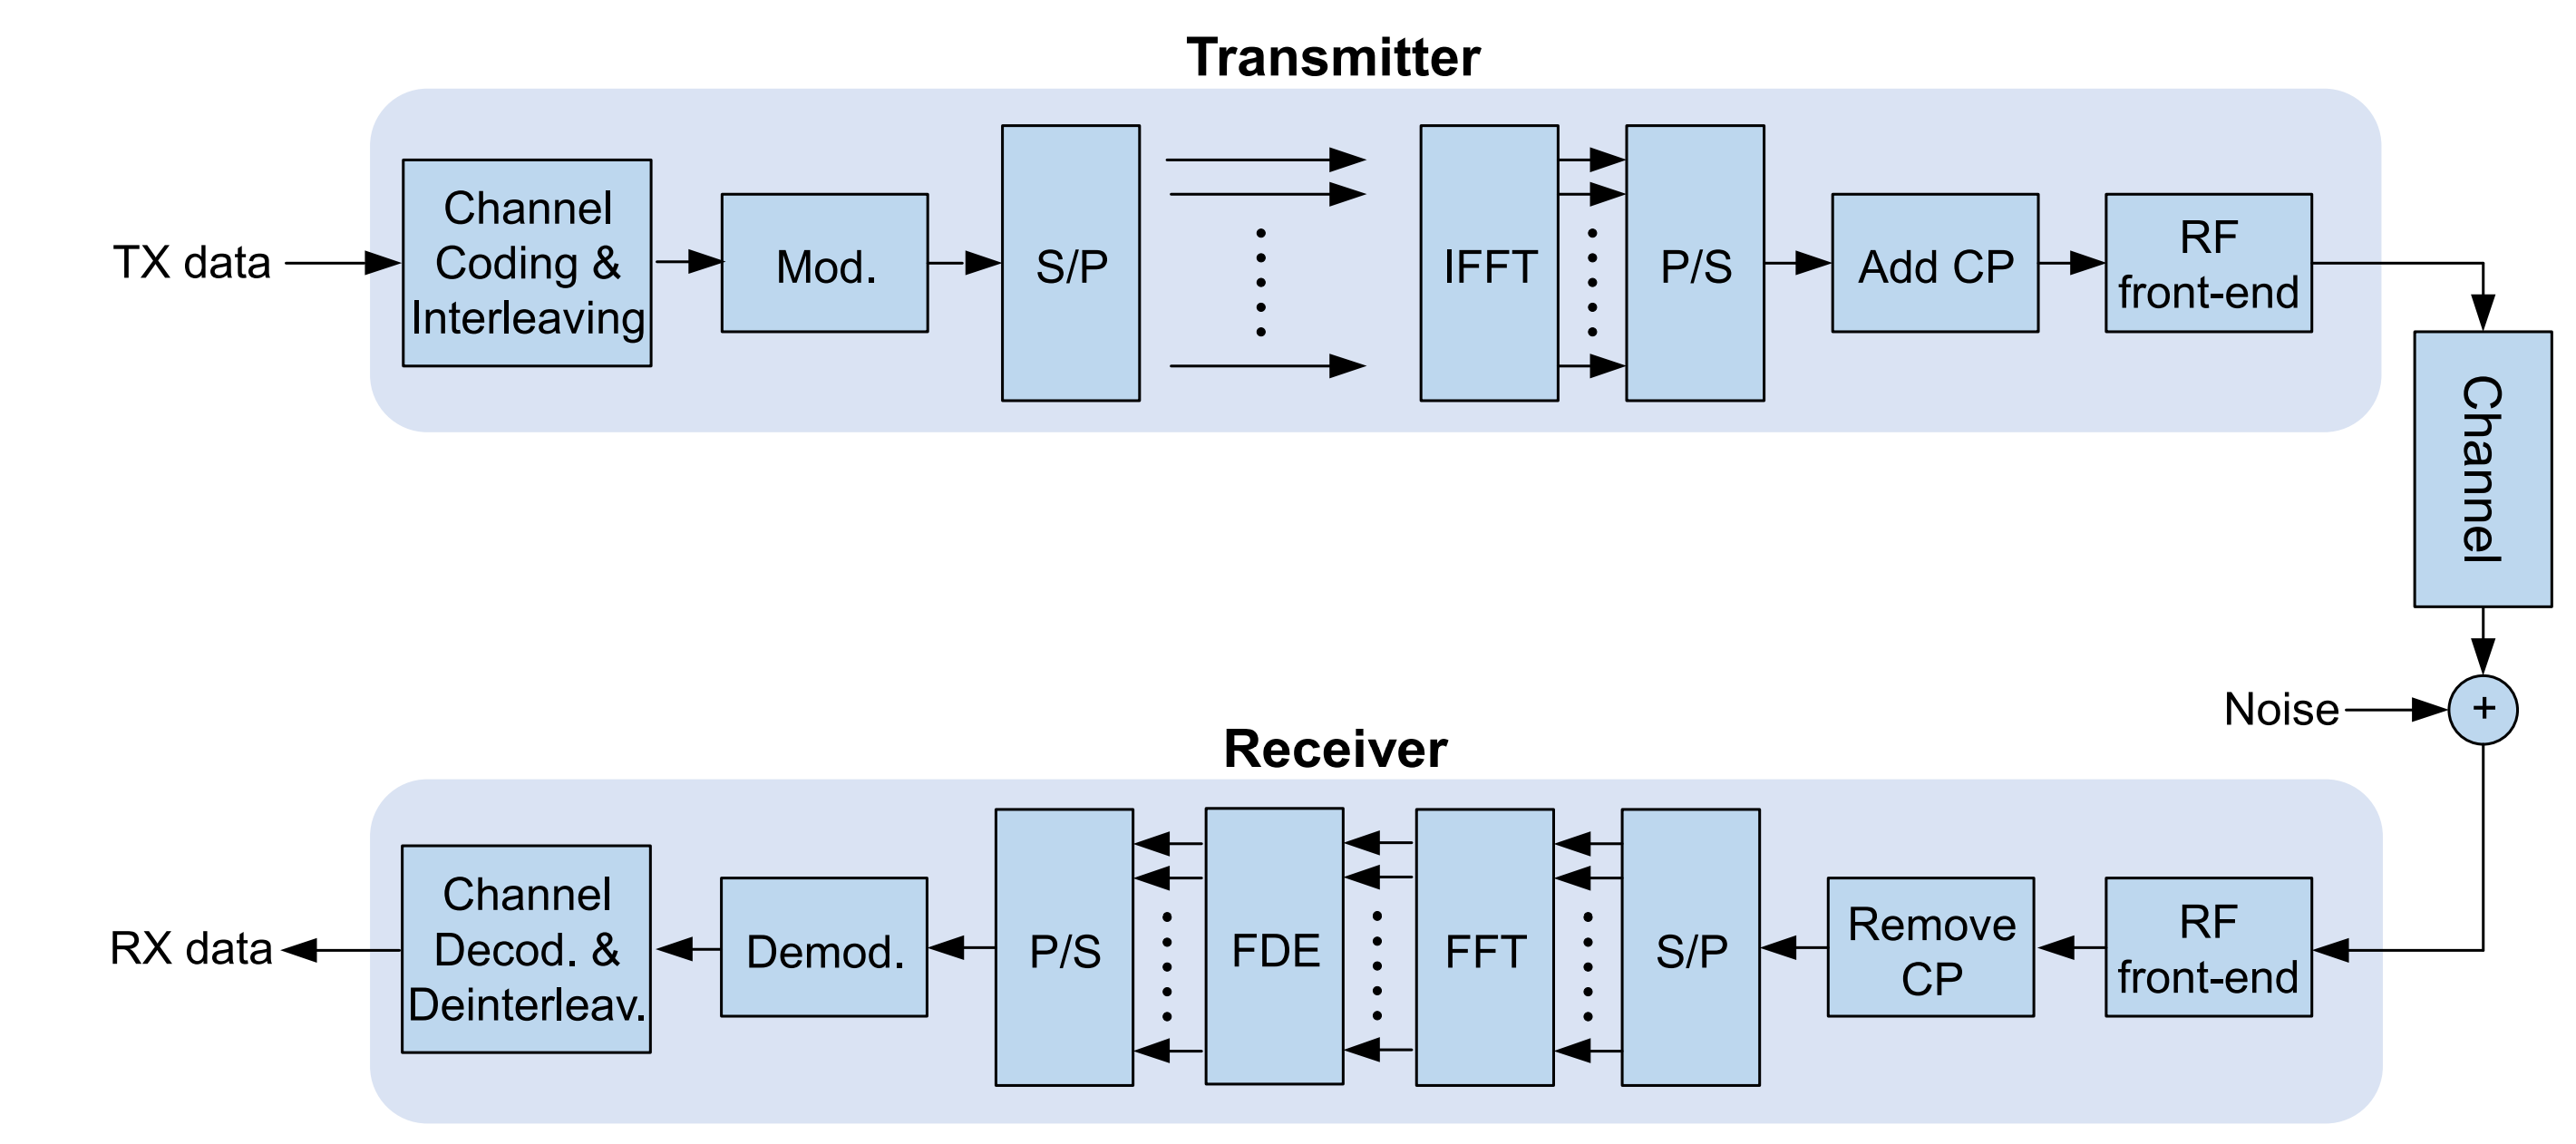
\includegraphics[width=\linewidth]{figs/ofdm_block.png}
\caption{Block diagram of a typical \gls{ofdm} system (image from~\cite{arslan2020flexible})}\label{fig:block_diagram}
\end{figure}

\section{The basics (in laymen terms)}\label{sec:ofdm-laymen}
Imagine you have a fast internet connection, and you want to send a large file to a friend. Instead of sending the entire file in one go, you decide to break it into smaller chunks and send them separately. This makes it easier to manage and lessens the chance of losing all the data if something goes wrong during transmission. This is the main operating principle of \gls{ofdm}.

\subsection{Key features}

\begin{itemize}
    \item[]\textbf{Frequency Division Multiplexing}\\ \Gls{ofdm} combines the principles of multiplexing and modulation. Multiplexing is the technique of combining multiple signals into one signal for transmission, while modulation involves modifying the properties of a carrier signal to encode information. In \gls{ofdm}, each subchannel is modulated independently using a technique like \gls{qam} (see \cref{sec:cohmod}), and then all the modulated subchannels are combined for transmission.
    \item[]\textbf{Orthogonality}\\
In \gls{fdm}, the subchannels are typically close to each other in frequency, which can lead to interference. \gls{ofdm} employs a clever technique called orthogonalization\footnote{In mathematics, two functions are orthogonal if their inner product (the integral of their product over a given interval) is zero.}, where the subchannels are spaced apart at precise intervals, ensuring that they don't interfere with each other. It's akin to having lanes on a highway spaced far enough apart that cars in one lane don't disrupt those in adjacent lanes.
\item[]\textbf{Multiplexing}\\
After orthogonalization, multiple streams of data can be transmitted simultaneously over the different subchannels. Each subchannel acts as a separate communication path, allowing for efficient use of the available spectrum. If the subchannels are used by multiple users, this technique is called \gls{ofdma}.
\end{itemize}

\subsection{Benefits of OFDM}

\begin{itemize}
    \item[] \textbf{Spectral Efficiency}\\
    By dividing the available bandwidth into smaller subchannels, \gls{ofdm} allows for efficient use of the spectrum. This enables higher data rates compared to traditional single-carrier modulation techniques.
    \item[] \textbf{Robustness}\\
    \Gls{ofdm} is inherently robust against frequency-selective fading~\cite{MCMorelli}, which occurs when different frequencies in the signal experience different levels of attenuation or delay. Since \gls{ofdm} divides the signal into multiple subchannels, even if some subchannels are affected by fading, others may still carry useful data.
    \item[] \textbf{Flexibility}\\
    \Gls{ofdm} can adapt to changing channel conditions by adjusting parameters such as subchannel spacing and modulation scheme. This flexibility makes it suitable for a wide range of communication systems.
\end{itemize}


\section{The OFDM System}\label{sec:ofdm-overview}

The block diagram of a typical \gls{ofdm} system is shown in~\cref{fig:block_diagram}. The main idea behind \gls{ofdm} is to divide a high-rate encoded data stream (with symbol time $T_S$) into $N$ parallel substreams (with symbol time $T = NT_S$) that are modulated onto $N$ orthogonal carriers (referred to as subcarriers). This operation is easily implemented in the discrete time domain through an $N$-point \gls{idft} unit and the result is transmitted serially. At the receiver, the information is recovered by performing a \gls{dft} on the received block of signal samples.
%

%
%
The data transmission in \gls{ofdm} systems is accomplished in a symbolwise fashion, where each OFDM symbol conveys~$N$ (possibly coded) complex data symbols. 

\subsection{The Wireless Channel -- A short summary}
In wireless communication systems, transmitted signals are typically reflected, diffracted, and scattered, arriving at the receiver along multiple paths with different delays, amplitudes, and phases as illustrated in~\cref{fig:multipath}. This leads to an overlapping of different copies of the same signal on the receiver side differing in their amplitude, time of arrival and phase. 
%
\begin{figure}[htbp]
\centering
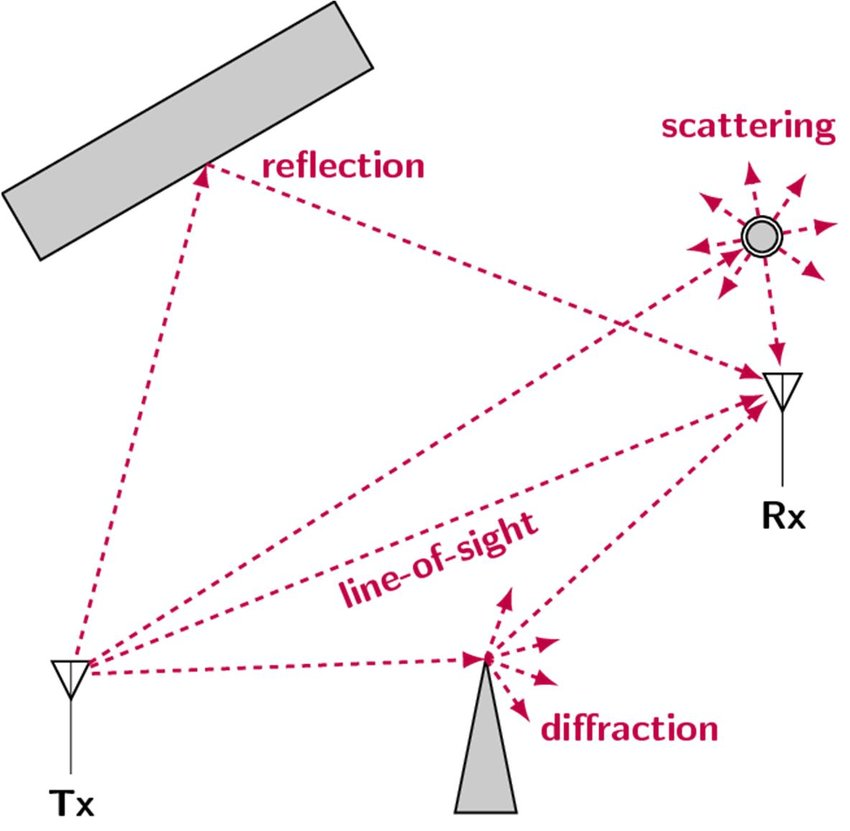
\includegraphics[width=0.4\textwidth]{figs/Some-effects-causing-multipath-propagation.png}
\caption{The basic principle of multipath propagation (image form~\cite{milosevic2021key})}\label{fig:multipath}
\end{figure}
%
A common model to describe the wireless channel makes use of the \textit{channel impulse response} (time domain), written as,
\begin{equation}
h(l)=\alpha(l) e^{j\theta(l)},
\end{equation} for $l = 0,\ldots,L-1 $, where $L$ presents the total number of received signal paths, while $\alpha(l)$ and $ \theta(l)$ are attenuation and phase shift of the $l$th path, respectively. The differences in the time of arrival are eliminated by the cyclic prefix, which is described in the next section. One of the effects of the reception of multiple overlapping copies, i.e., multipath, is frequency selective fading. From the signal's perspective, the signal experiences different attenuation for different frequencies, complicating mitigation of these unwanted effects. This is the reason why \gls{ofdm} is used, as it ''splits'' the spectrum in several subchannels, allowing to use single-tap equalizers to resolve frequency-selective fading. See~\cref{ss:equ} for more details.


As a consequence of the time dispersion associated with the frequency-selective channel, contiguous \gls{ofdm} symbols may partially overlap in time-domain. This phenomenon results into \gls{isi}, with ensuing limitations of the system performance. The common approach to mitigate \gls{isi} is to introduce a guard interval of appropriate length between adjacent symbols. In practice, the guard interval is obtained by duplicating the last part of the \gls{ofdm} symbol and, for this reason, is commonly referred to as \gls{cp}.
As illustrated in~\cref{fig:cp}, the \gls{cp} is appended in front of the corresponding \gls{idft} output. This results into an extended \gls{ofdm} symbol consisted of the \gls{cp} and original \gls{ofdm} symbol. The \gls{isi} can be removed as long as the \gls{cp} length is properly designed according to the channel delay spread.

Referring to~\cref{fig:block_diagram}, lets concentrate on the receiver. The first operation is the \gls{cp} removal, which is simply accomplished by discarding the first $N_G$ samples of the considered segment (the lenght of the \gls{cp}). The remaining $N$ samples are fed to a \gls{dft} and the corresponding output is subsequently passed to the \gls{fde}. Assuming that synchronization has already been established and the \gls{cp} is sufficiently long to eliminate the \gls{isi}, only a one-tap complex-valued multiplier is required to compensate for the channel distortion over each subcarrier, which will be further described in~\cref{ss:equ}. To better understand this fundamental property of \gls{ofdm}, however, we need to introduce the mathematical model of the communication scheme depicted in ~\cref{fig:block_diagram}.
%
\begin{figure}[thb]
\centering
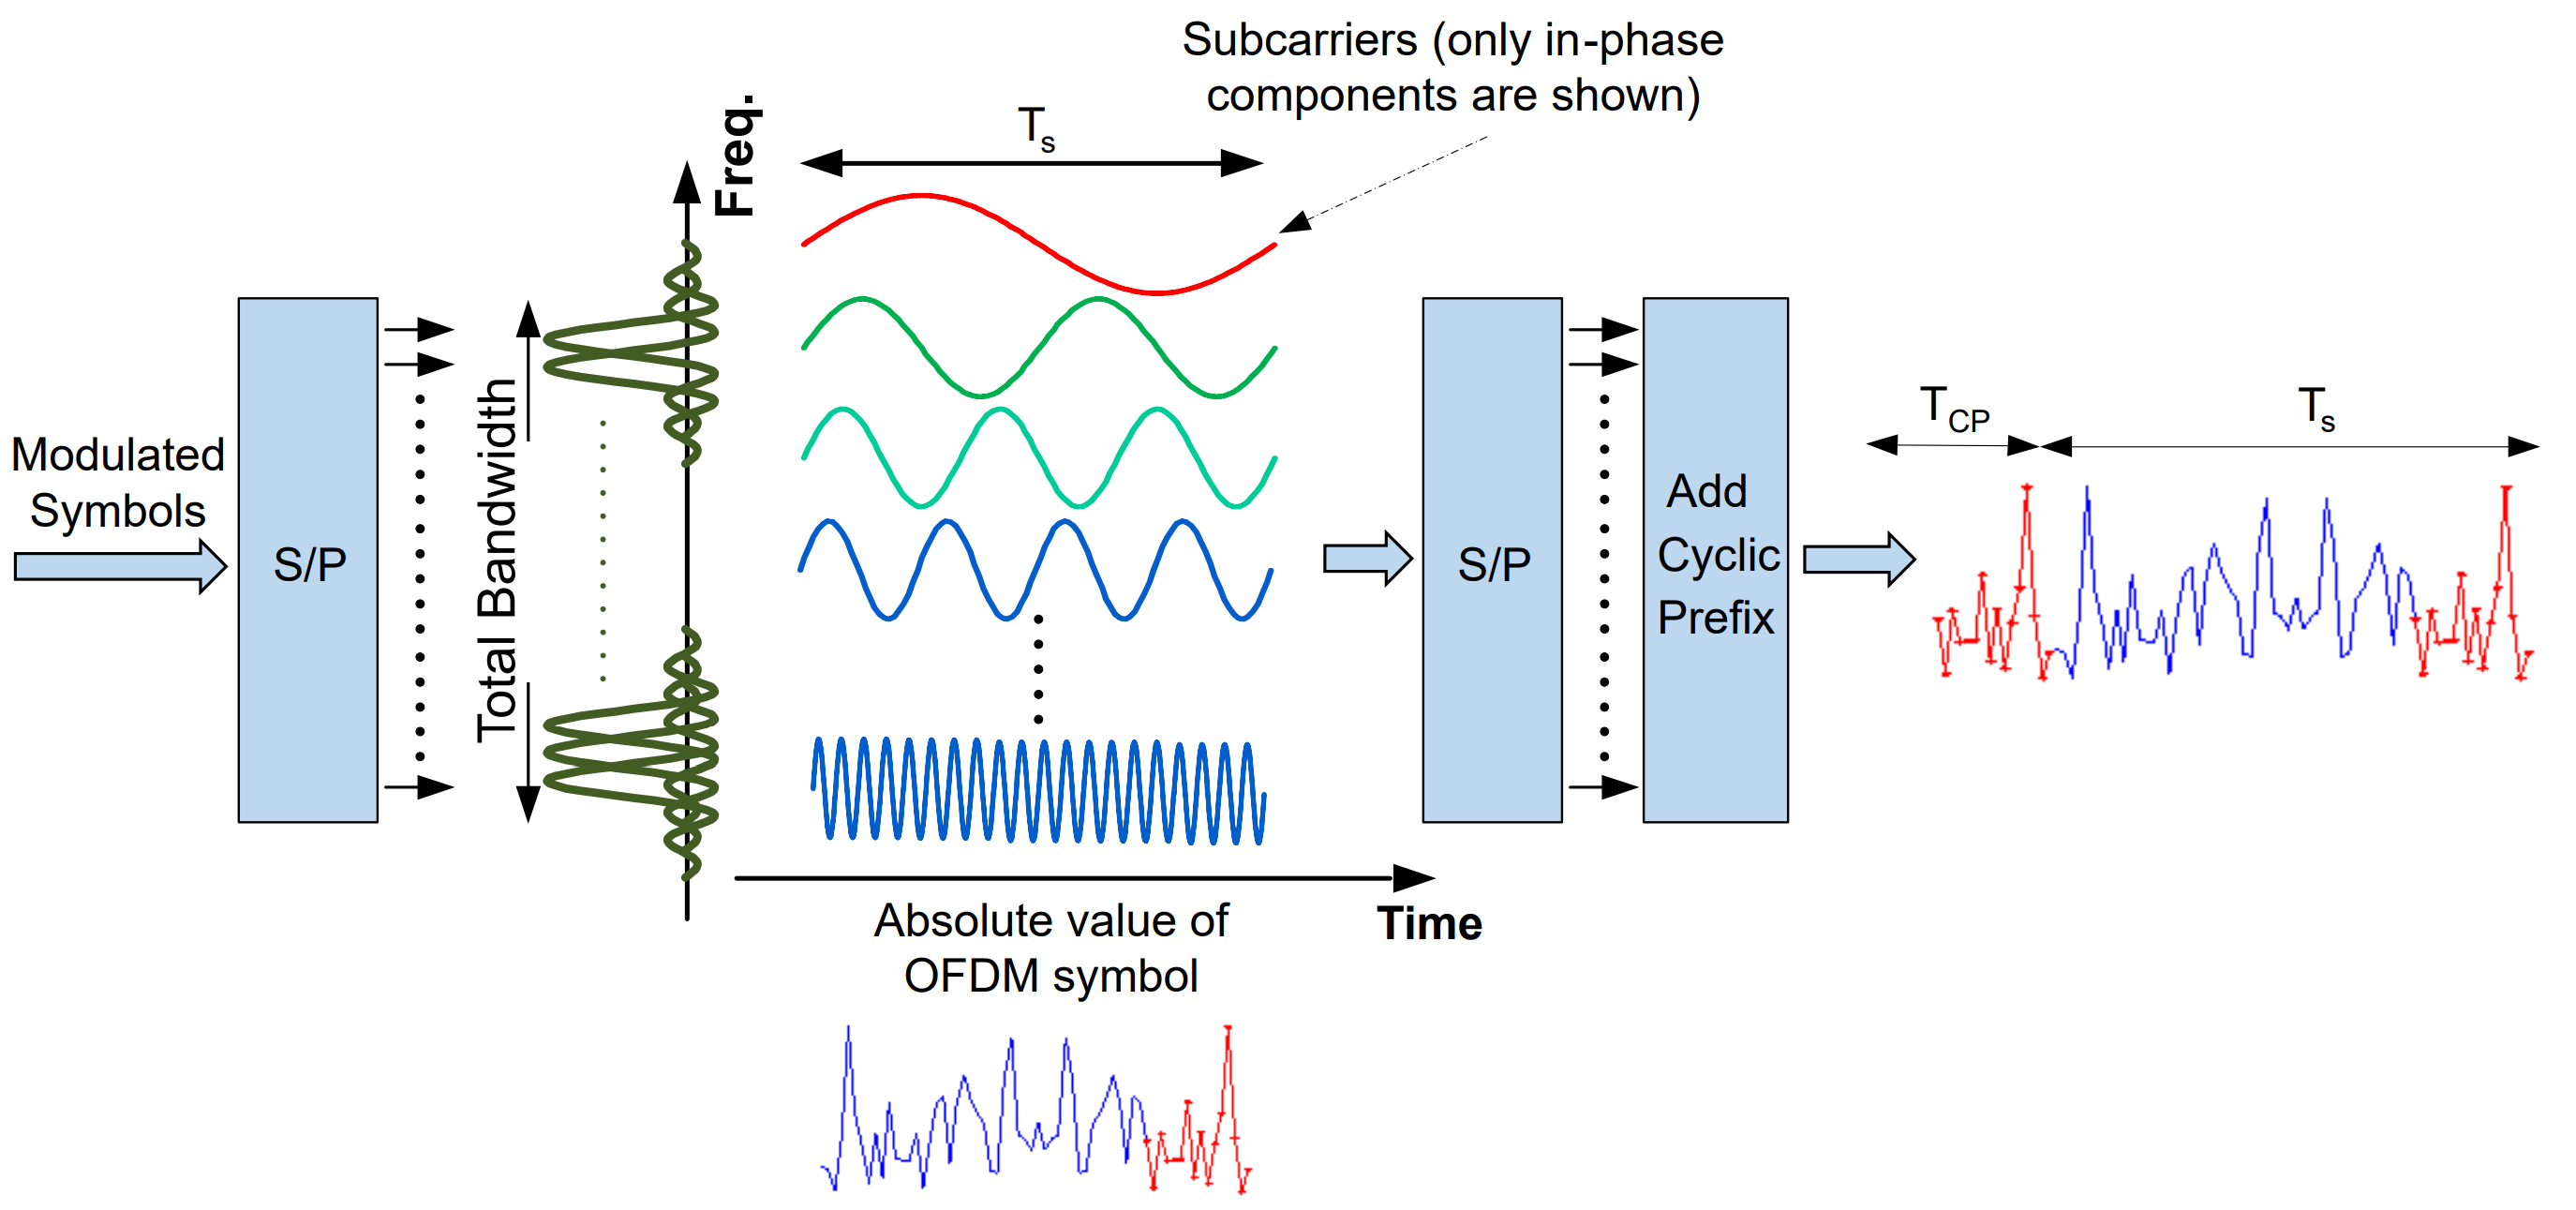
\includegraphics[width=1.00\linewidth]{figs/cp-ofdm_block.png}
\caption{Structure of an OFDM symbol (image from~\cite{arslan2020flexible})}\label{fig:cp}
\end{figure}



\section{Discrete-time OFDM System Model}\label{sec:discmod}

Since \gls{ofdm} is a block based communication model, a serial data stream is converted into parallel blocks of size N and \gls{idft} is applied to obtain time-domain \gls{ofdm} symbols. 
% Let denote $\mathbf{C_i}=\left[ C_i(0),C_i(1),\dots,C_i(N-1)\right]^T$ the $i$th block of data at the IDFT input, with length $N$ where $(.)^T$ represents the transponse operator. 
Complex data symbols $C_i(n)$, for $n=0,\ldots,N-1$, within the $i$th OFDM symbol are taken from either a \gls{psk} or \gls{qam} constellation. Then, time domain representation of the $i$th OFDM symbol after \gls{idft} and \gls{cp} insertion is given by
%
\begin{equation}\label{IDFT}
c_i(k)= 
\begin{cases}
   \sum_{n=0}^{N-1}{C_i(n)e^{j2\pi kn/N}},& -N_G \leq k \leq N-1\\
   0,&\text{else}
\end{cases},
\end{equation}
%
where $N_G$ is the length of the \gls{cp} which is an important design parameter of the \gls{ofdm} system that defines the maximum acceptable length of channel impulse response. Furthermore, the transmitted signal can be obtained by concatenating \gls{ofdm} symbols in time domain as

\begin{equation}\label{concat}
c(k)=\sum_i{c_i(k -iN_T)}.
\end{equation} 

In addition to multipath effects, additive noise is introduced to the transmitted signal. The main sources of additive noise are thermal background noise, electrical noise in the receiver amplifiers, and interference \cite{StuberOFDM}. The noise decreases the \gls{snr} of the received signal, resulting in a decreased performance. The total effective noise at the receiver of an \gls{ofdm} system can be modeled as \gls{awgn} with a uniform spectral density and zero-mean Gaussian probability distribution. The time domain noise samples are represented by $w(k) \sim CN(0,\sigma_w^2)$, where $\sigma_w^2$ denotes the noise variance and $0$ the mean of the circular symmetric complex distribution. Therefore, the discrete-time model of received \gls{ofdm} signals can be written as,
\begin{equation}
\label{eqn:multipath}
y(k) = \sum_{l = 0}^{L-1} h(l)c(k-l) + w(k).
\end{equation}
%
Multipath propagation and additive noise affect the signal significantly, corrupting the signal and often placing limitations on the performance of the system.








\section{OFDM System Impairments}\label{sec:sysimp}
Since timing and frequency errors in multi-carrier systems destroy orthogonality among subcarriers which results in large performance degradations, synchronization of time and frequency plays a major role in the design of a digital communication system. Essentially, this function aims at retrieving some reference parameters from the received signal that are necessary for reliable data detection. In an \gls{ofdm} system, the following synchronization tasks can be identified \cite{MCMorelli}:
\begin{itemize}
 \item \textit{sampling clock synchronization}: in practical systems the sampling clock frequency at the receiver is slightly different from the corresponding frequency at the transmitter. This produces \gls{ici} at the output of the receiver's \gls{dft} with a corresponding degradation of the system performance. The purpose of a sampling clock synchronization is to limit this impairment to a tolerable level.
\item \textit{timing synchronization}: the goal of this operation is to identify the starting point of each received OFDM symbol in order to find the correct position of the \gls{dft} window. In burst-mode transmissions timing synchronization is also used to locate the start of the frame (frame synchronization) which is a collection of OFDM symbols.
\item \textit{frequency synchronization}: a frequency error between the local oscillators at the transmitter and receiver results in a loss of orthogonality among subcarriers with ensuing limitations of the system performance. Frequency synchronization aims at restoring orthogonality by compensating for any frequency offset caused by oscillator inaccuracies.
% or Doppler shifts.
\end{itemize}

The block diagram of the receiver is depicted in~\cref{fig:receiver}. In the analog frontend, the incoming waveform $r_{RF}(t)$ is filtered and down-converted to baseband using two quadrature sinusoids generated by a \gls{lo}. The baseband signal is then passed to the \gls{adc}, where it is sampled with frequency $f_s = 1/T_s$. Due to Doppler shifts and/or oscillator instabilities, the frequency $f_{LO}$ of the \gls{lo} is not exactly equal to the received carrier frequency $f_c$. The difference $f_d = f_c - f_{LO}$ is referred to as \gls{cfo}, or shorter frequency offset, causing a phase shift of $2\pi kf_d$\footnote{Notice that this phase shift is not time dependent (if $f_d$ is constant) and is different for each subcarrier $k$.}. Therefore, the received baseband signal can be expressed as
%
\begin{equation}
\label{eqn:received_time_freqshift}
r(k) =y(k)e^{j2\pi \varepsilon k/N} 
\end{equation}
%
where

\begin{equation}
\label{eqn:norm_freq_off}
\varepsilon = Nf_dT_s
\end{equation}

is the frequency offset normalized to subcarrier spacing $\Delta f =1/(NT_s)$.
In addition, since the time scales at the transmitter and the receiver are not perfectly aligned, at the start-up the receiver does not know where the OFDM symbols start and, accordingly, the \gls{dft} window will be placed in a wrong position. As it will be shown later, since small (fractional) timing errors do not produce any degradation of the system performance, it suffices to estimate the beginning of each received OFDM symbol within one sampling period.
%
\begin{figure}[thb]
\centering
\includegraphics[width=1.00\linewidth]{syncstages.eps}
\caption{Block diagram of a basic OFDM receiver\label{fig:receiver} }
\end{figure}
%
Let $\Delta k$ denotes the number of samples by which the receive time scale is shifted from its ideal setting. The samples from ADC are thus expressed by
%
\begin{equation}
\label{eqn:received_time_frtime}
r(k) =e^{j2\pi \varepsilon k/N}y(k-\Delta k) + w(k).
\end{equation}
%
Replacing (\ref{concat}) and (\ref{eqn:multipath}) in (\ref{eqn:received_time_frtime}), samples are given as
%
\begin{equation}
\label{eqn:received_time_all}
r(k) =e^{j2\pi \varepsilon k/N} \sum_i{}\sum_{l=0}^{L-1}{h(l)c_i(k-l-\Delta k-iN_T)}+ w(k).
\end{equation}

The frequency and timing synchronization units shown in ~\cref{fig:receiver} employ the received samples $r(k)$ to compute estimates of $\varepsilon$ and $\Delta k$, noted as $\hat{\varepsilon}$ and $\hat{\Delta k}$. The former is used to counter-rotate $r(k) $ at an angular speed $2\pi \hat{\varepsilon} k/N$ (frequency correction) using \gls{cfo}, while the timing estimate is exploited to achieve the correct position of the received signal within the \gls{dft} window (timing correction). Specifically, the samples $r(k)$ with indices $iN_T + \Delta k \leq k \leq iN_T + \Delta k + N - 1$ are fed to the \gls{dft} device and the corresponding output is used to detect the data symbols conveyed by the $i$th OFDM block.
%The DFT output can also be exploited to track and compensate for small short-term variations of the frequency error (fine-frequency estimation).
\subsection{Effects of Frequency Offset}

In order to assess the impact of a frequency error on the system performance, we assume ideal timing synchronization and let $\Delta k = 0$ and $N_g \geq L-1$.
At the receiver, the \gls{dft} output for the $i$th OFDM symbol is computed as
%
\begin{equation}
\label{eqn:received_freq_freqoff}
R_i(n) =\frac{1}{N} \sum_{k=0}^{N-1} r(k+iN_T)e^{-j2\pi k n/N} ,\ 0 \leq n \leq N-1
\end{equation}
%
Substituting (\ref{eqn:received_time_all}) into (\ref{eqn:received_freq_freqoff}) we get
%
\begin{equation}
\label{eqn:received_freq_devel}
\begin{split}
R_i(n)
&=\frac{1}{N}\sum_{k=0}^{N-1}{\left[ e^{j2\pi \varepsilon(k+iN_T)/N}\sum_{l=0}^{L-1} {h(l)c_i(k-l)}+w(k)\right] e^{-j2\pi kn/N}}\\
&=\frac{1}{N}e^{j\varphi_i}\sum_{k=0}^{N-1}{e^{j2\pi k(\varepsilon-n)/N}}\sum_{l=0}^{L-1} {h(l)\sum_{m=0}^{N-1}{C_i(m)e^{j2\pi (k-l)m/N}}}+W_i(n)\\
&=\frac{1}{N}e^{j\varphi_i} \sum_{m=0}^{N-1} \left\lbrace \sum_{l=0}^{L-1} h(l)e^{j2\pi lm/N}\right\rbrace C_i(m)\sum_{k=0}^{N-1} e^{-j2\pi k (m+\varepsilon -n)/N}+W_i(n)\\
&=\frac{1}{N}e^{j\varphi_i} \sum_{m=0}^{N-1} H(m) C_i(m)\sum_{k=0}^{N-1} e^{j2\pi k (m+\varepsilon -n)/N} +W_i(n)
\end{split}
\end{equation}
%
%
where $\varphi_i = 2\pi i \varepsilon N_T/N$, $W_i(n)$ is Gaussian distributed thermal noise with variance $\sigma_{w}^2$ derived as
%
\begin{equation}
\label{eqn:noise_freq}
W_i(n) =\frac{1}{N} \sum_{k=0}^{N-1} w(k)e^{-j2\pi k n/N} ,\ 0 \leq n \leq N-1
\end{equation}
%
and $H(m)$ is {channel frequency response}\index{Channel frequency response} defined as DFT of channel impulse response given as
%
\begin{equation}
\label{eqn:CFR}
H(m) =\sum_{l=0}^{L-1} h(l)e^{-j2\pi l m/N} ,\ 0 \leq m \leq N-1.
\end{equation}
%
Performing standard mathematical manipulations (\ref{eqn:received_freq_devel}) is derived to
%
\begin{equation}
\label{eqn:received_freq_developed}
R_i(n)=e^{j\varphi_i} \sum_{m=0}^{N-1} H(m) C_i(m)f_N(\varepsilon + m - n)e^{j\pi (N-1)(\varepsilon +m - n)/N} +W_i(n),
\end{equation}
%
where
%
\begin{equation}
\label{eqn:fN}
\begin{split}
f_N(x)
&= \frac{\sin(\pi x)}{N\sin(\pi x/N)}\\
&\approx \frac{\sin(\pi x)}{\pi x} = \operatorname{si}(\pi x)
\end{split}
\end{equation}
%
can be derived using the standard approximation $sin(t)\approx t$ for small values of argument $t$.

In the case when the frequency offsetis a multiple of subcarrier spacing $\Delta f$, i.e., $\varepsilon$ is integer-valued, (\ref{eqn:received_freq_developed}) reduces to
%
\begin{equation}
\label{eqn:received_freq_developed_integer}
R_i(n)=e^{j\varphi_i} H({|n-\varepsilon|}_N)C_i({|n-\varepsilon|}_N) +W_i(n),
\end{equation}
%
where ${|n-\varepsilon|}_N$ is the value of $n-\varepsilon$ reduced to interval $\left[ 0,N-1\right)$. This equation indicates that \textbf{an integer frequency offset does not destroy orthogonality among subcarriers and only results into a shift of the subcarrier indices by a quantity} $\varepsilon$. In this case the $n$th DFT output is an attenuated and phase-rotated version of $C_i({|n-\varepsilon|}_N)$ rather than of $C_i(n)$. Otherwise, when $\varepsilon$ is not integer-valued the subcarriers are no longer orthogonal and \gls{ici} does occur. In this case it is convenient to rewrite (\ref{eqn:received_freq_developed}) like
%
\begin{equation}
\label{eqn:received_freq_developed_noninteger}
R_i(n)=e^{j\left[ \varphi_i + \pi\varepsilon (N-1)/N\right] } H(n)C_i(n)f_N(\varepsilon) + I_i(n,\varepsilon) +W_i(n),
\end{equation}
%
where $I_i(n,\varepsilon)$ accounts for ICI and is given as
%
\begin{equation}
\label{eqn:Ii}
I_i(n,\varepsilon)=e^{j\varphi_i} \sum_{m=0,m \neq n}^{N-1} H(m) C_i(m)f_N(\varepsilon + m - n)e^{j\pi (N-1)(\varepsilon +m - n)/N}.
\end{equation}
%
From (\ref{eqn:received_freq_developed_noninteger}) it follows that non-integer normalized frequency offset$\varepsilon$ influences the received signal on $n$th subcarrier twofold.
Firstly, received signals on all subcarriers are \textbf{equally} attenuated by $f_n^2(\varepsilon)$ and phase shifted by $(\varphi_i + \pi\varepsilon (N-1)/N)$, while the second addend in (\ref{eqn:received_freq_developed_noninteger}) presents interference from other subcarriers (\gls{ici}).

Letting $E\left\lbrace |H(n)|^2\right\rbrace =1$ and assuming independent and identically distributed data symbols with zero mean and power $S = E\left\lbrace |C_i(n)|^2\right\rbrace =1$, the interference term $I_i(n,\varepsilon)$ can reasonably be modeled as a Gaussian zero-mean random variable with variance (power) defined as
%
%
\begin{equation}
\label{eqn:Ii_variance}
 \sigma_i^2(\varepsilon)= E\left\lbrace |I_i(n)|^2\right\rbrace=S\sum_{\substack{{m=0}\\{m\neq n}}}^{N-1}f_N^2(\varepsilon + m - n).
\end{equation}
%
Under assumption that all subcarriers are used and by means of the identity
%
\begin{equation}
\label{eqn:Ii_identity}
\sum_{m=0}^{N-1}f_N^2(\varepsilon + m - n) = 1,
\end{equation}
%
which holds true independently of $\varepsilon$, interference power (\ref{eqn:Ii_variance}) can be written as
%
\begin{equation}
\label{eqn:Ii_simmpl}
 \sigma_i^2(\varepsilon)=S\left[ 1 - f_N^2(\varepsilon)\right] .
\end{equation}
%
A useful indicator to evaluate the effect of frequency offset on the system performance is the loss in \gls{snr}, which is defined as
%
\begin{equation}
\label{eqn:SNRloss}
 \gamma(\varepsilon) = \frac{SNR^{(ideal)}}{SNR^{(real)}},
\end{equation}
%
where $SNR^{(ideal)}$ is the \gls{snr} of a perfectly synchronized system given as
%
\begin{equation}
\label{eqn:SNRideal}
 SNR^{(ideal)} = S/\sigma_w^2 = E_S/N_0,
\end{equation}
%
where $E_S$ is the average received energy over each subcarrier while $N_0/2$ is the two-sided power spectral density of the ambient noise, while 
%
\begin{equation}
\label{eqn:SNRreal}
 SNR^{(real)} = S f_N^2(\varepsilon)/\left[ \sigma_w^2 + \sigma_i^2(\varepsilon)\right],
\end{equation}
%
is the \gls{snr} in the presence of a frequency offset $\varepsilon$. Substituting (\ref{eqn:SNRideal}) and (\ref{eqn:SNRreal}) into (\ref{eqn:SNRloss}), it becomes
%
\begin{equation}
\label{eqn:SNRlossdevel}
 \gamma(\varepsilon) = \frac{1}{f_N^2(\varepsilon)}\left[ 1+\frac{E_S}{N_0}(1-f_N^2(\varepsilon))\right].
\end{equation}
%
For small values of $\varepsilon$ (\ref{eqn:SNRlossdevel}) can be simplified using the Taylor series expansion of $f_N^2(\varepsilon)$ around $\varepsilon = 0$, resulting in
%
\begin{equation}
\label{eqn:SNRlossdevelapprox}
 \gamma(\varepsilon) \approx 1 + \frac{1}{3} \frac{E_S}{N_0} {(\pi \varepsilon)}^2.
\end{equation}
%
It can be seen that the \gls{snr} loss is approximately proportional to the square of the normalized frequency offset$\varepsilon$.

\subsection{Effects of Timing Offset}

In order to assess the performance of the \gls{ofdm} system in the presence of small \gls{to} let assume perfect frequency synchronization, i.e., $\varepsilon = 0$ and consider only the effect of \gls{to} when it is smaller than the uncorrupted part of the cyclic prefix, i.e., $\Delta k \leq N_g - (L + 1)$.

Under these assumptions, (\ref{eqn:received_freq_freqoff}) is derived to
%
\begin{equation}
\label{eqn:received_time_devel}
\begin{split}
R_i(n)
&=\frac{1}{N} \sum_{k=0}^{N-1} \left[ \sum_{l=0}^{L-1}h(l)c_i(k-l-\Delta k) + w_i(k)\right] e^{-j2\pi k n /N}\\
&=\frac{1}{N} \sum_{k=0}^{N-1} \sum_{l=0}^{L-1}h(l)\sum_{m=0}^{N-1}{C_i(m)e^{j2\pi (k-l -\Delta k)m/N}} e^{-j2\pi k n /N}+W_i(n)\\
&=\frac{1}{N} \sum_{m=0}^{N-1} \left[ \sum_{l=0}^{L-1} h(l)e^{-j2\pi lm/N}\right] C_i(m)\left[ \sum_{k=0}^{N-1} e^{-j2\pi k (m-n)/N}\right]e^{-j2\pi \Delta k m/N} +W_i(n)\\
&=\sum_{m=0}^{N-1} H(m) C_i(m)\delta(m-n)e^{-j2\pi \Delta k m/N} +W_i(n)\\
&= H(n) C_i(n)e^{-j2\pi \Delta k m/N} +W_i(n),
\end{split}
\end{equation}
%
%
where $W_i(n)$ and $H(m)$ are defined in (\ref{eqn:noise_freq}) and (\ref{eqn:CFR}), respectively, while $\delta(m-n)$ presents the Kronecker delta defined as
%
\begin{equation}
\label{eqn:CrDel}
\delta(m-n) = 
\begin{cases}
   1,&m = n\\
   0,&m\neq n.
\end{cases}.
\end{equation}
%
From expression above it can be seen that small \gls{to} causes only a linear phase rotation across the \gls{dft} outputs and can be compensated by the channel equalizer, which can not distinguish between phase shifts introduced by the channel and those derived from the \gls{to}. Timing offset does not destroy the orthogonality of the carriers and the effect of timing error is a phase rotation which linearly changes with subcarrier order.

\subsection{Equalization}\label{ss:equ}

Channel equalization is the process through which a coherent receiver compensates for any distortion induced by frequency-selective fading. For the sake of simplicity, ideal timing and frequency synchronization is considered throughout this subsection. The channel is assumed static over each \gls{ofdm} block, but can vary from block to block. Under these assumptions, and assuming that the receiver is perfectly synchronized, i.e, $\varepsilon = 0$ and $\Delta k = 0$, the output of the receiver's \gls{dft} unit during the $i$th symbol is given by
%
\begin{equation}
\label{eqn:DFTout}
 R_i(n)=H_i(n)C_i(n) + W_i(n),\ 0\leq n \leq N-1
\end{equation}
%
where $C_i(n)$ is the complex data symbol and $W_i(n)$ as well as $H(m)$ are defined in (\ref{eqn:noise_freq}) and (\ref{eqn:CFR}), respectively. An important feature of \gls{ofdm} is that channel equalization can independently be performed over each subcarrier by means of a bank of one-tap multipliers. As shown in ~\cref{fig:equalization}, the $n$th \gls{dft} output $R_i(n)$ is weighted by a complex-valued coefficient $P_i(n)$ in order to compensate for the channel-induced attenuation and phase rotation. The equalized sample $Y_i(n)=P_i(n)R_i(n)$ is then subsequently passed to the detection unit, which delivers final decisions $\hat{C}_i(n)$ on the transmitted data.
%
\begin{figure}[thb]
\centering
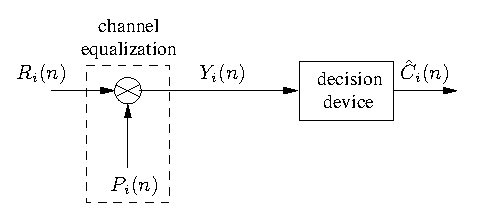
\includegraphics[width=0.6\linewidth]{equalization.eps}
\caption{Block diagram of an OFDM receiver\label{fig:equalization}}
\end{figure}
%
Intuitively, the simplest method for the design of the equalizer coefficients, is to perform a pure channel inversion, know as \gls{zf} criterion. The equalizer coefficients are then given by
%
\begin{equation}
\label{eqn:EqCoeff}
 P_i(n)=\frac{1}{H_i(n)},
\end{equation}
%
while the DFT output takes the form
%
\begin{equation}
\label{eqn:DFToutEq}
 Y_i(n)=\frac{R_i(n)}{H_i(n)}=C_i(n) + \frac{W_i(n)}{H_i(n)},\ 0\leq n \leq N-1.
\end{equation}
%
From (\ref{eqn:DFToutEq}) it can be noticed that ZF equalization is capable of totally compensating for any distortion induced by the wireless channel. However, the noise power at the equalizer output is given by $\sigma_w^2/|H_i(n)|^2$ and may be excessively large over deeply faded subcarriers characterized by low channel gains. 

Inherent system requirement for ZF equalizer is the knowledge of the channel transfer function $H_i(n)$. Therefore, in many wireless \gls{ofdm} systems, sequence of data symbols is preceded by several reference OFDM symbols (preambles) known to the receiver, forming the \textbf{OFDM frame}. Typical frame structure is shown in {~\cref{fig:frame}} where preambles are typically used for \textbf{synchronization} and/or \textbf{channel estimation} purposes.
%
\begin{figure}[thb]
\centering
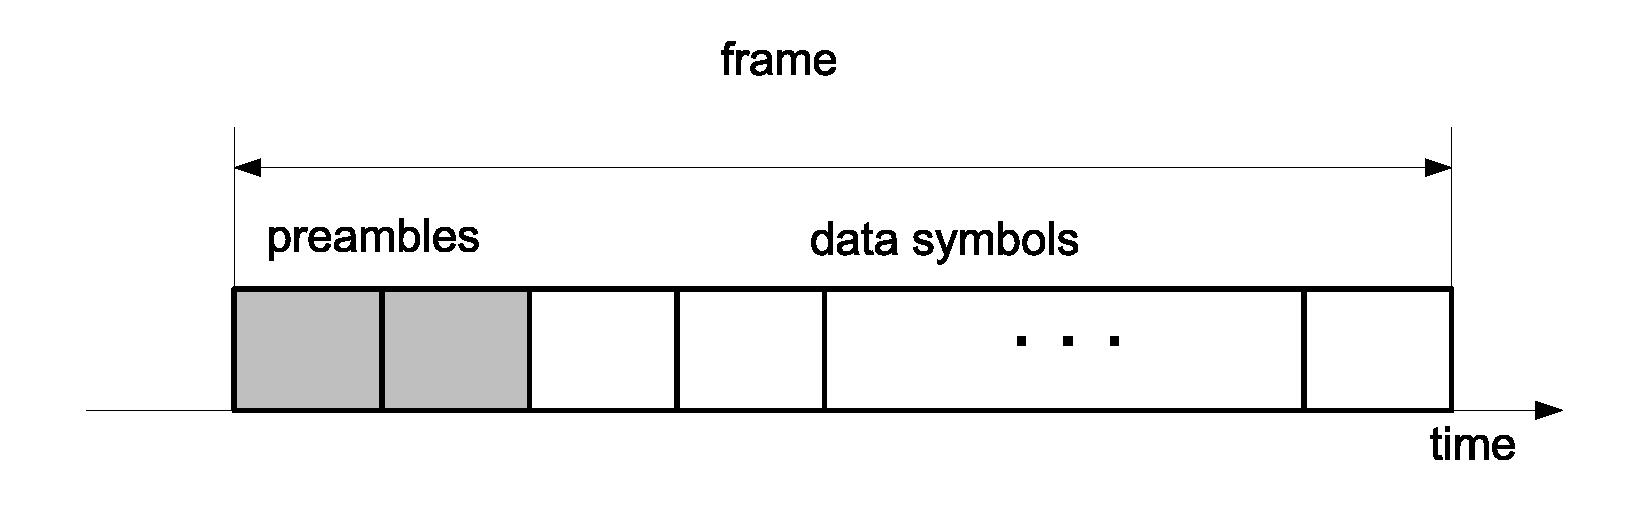
\includegraphics[width=0.6\linewidth]{framefinal}
\caption{Frame structure\label{fig:frame}}
\end{figure}
%
In typical fixed wireless standards as WLAN, it can be assumed that the channel remains static over frame duration, i.e., $H_i(n) = H(n)$ for $i = 1,\ldots,I$, where $I$ is the total number of OFDM symbols within one frame. Then, channel estimates obtained from the preambles can be used to coherently detect the entire payload.

Assuming that the OFDM frame has one preamble with index $i=p=1$, the output of the DFT block (\ref{eqn:DFTout}) can be written as
%
\begin{equation}
\label{eqn:DFToutPream}
 R_p(n)=H(n)C_p(n) + W_p(n),\ 0\leq n \leq N-1
\end{equation}
%
where $C_p(n)$ are complex data symbols \textbf{known} to the receiver. Then, estimates of the {channel frequency response}\index{Channel frequency response} $\hat{H}(n)$ can be obtained as
%
\begin{equation}
\label{eqn:Estimates}
 \hat{H}(n) = \frac{R_p(n)}{C_p(n)}=H(n) + \frac{W_p(n)}{C_p(n)},\ 0\leq n \leq N-1.
\end{equation}
%
On the other hand, in applications characterized by relatively high mobility as those envisioned by the \gls{lte} standard, the channel response undergoes significant variations over one frame and must continuously be tracked to maintain reliable data detection. In this case, in addition to initial reference blocks, known symbols called pilots are normally inserted into the payload section of the frame at some convenient positions. These pilots are scattered in both time and frequency directions (i.e., they are positioned over different blocks and different subcarriers), and are used as reference values for channel estimation and tracking.

In order to assess and compare the influence of system impairments on different data rates supported in \gls{ofdm} systems, a short survey of commonly used coherent modulation techniques and their performance evaluation in \gls{awgn} channel are given in the next section.

\section{Digital Modulations Used in OFDM Systems}\label{sec:cohmod}
%
Consider some digital information that is given by a finite bit sequence. To transmit this information over a physical, analog channel by a passband signal (on the \gls{rf} frequency) we need a mapping rule between the set of bit sequences and the set of possible signals or constellation points on the complex plane, as shown in ~\cref{fig:PSKconstell}. Such a mapping rule is called a digital modulation scheme. An example is shown in~\cref{fig:bpsk-passband}, where the red signal represent a logical $1$ and the blue signal a logical $0$. The signal frequency is the carrier frequency, i.e., it is the passband signal. In \acrlong{bb}, this would be represented by one complex symbol per passband signal. To go from the passband to the \gls{bb}, the carrier frequency is removed from the passband signal, thus the only thing remaining is the amplitude and phase contributions, i.e., the complex symbol. 

\begin{figure}
    
    \begin{subfigure}[t]{0.6\textwidth}
    \centering
    \begin{tikzpicture}
  % Parameters
  \def\phaseA{180} % Phase in degrees for cosine A
  \def\phaseB{0} % Phase in degrees for cosine B
  \def\frequencyA{2} % Frequency in Hz for cosine A
  \def\frequencyB{2} % Frequency in Hz for cosine B
  \def\amplitudeA{1} % Amplitude for cosine A
  \def\amplitudeB{1} % Amplitude for cosine B
  
  % Plot cosine function A
  \draw[->] (0,-2) -- (6.8,-2) node[right] {$t$};
  \draw[->] (0,-2) -- (0,2) node[above] {$y$};
  \draw[domain=0:2*pi,samples=200,smooth,variable=\t,blue] plot ({\t},{\amplitudeA*cos(\frequencyA*\t r + \phaseA)});
  
  % Plot cosine function B
  \draw[domain=0:2*pi,samples=200,smooth,variable=\t,red] plot ({\t},{\amplitudeB*cos(\frequencyB*\t r + \phaseB)});


  \node[right, red] at (2*pi,1) {$1$};
  \node[right, blue] at (2*pi,-1) {$0$};

  \node[below] at (2*pi,-2) {$T$};
  
   \node[below] at (0,-2) {$0$};
  % Vertical dashed line at t = 2*pi
  \draw[dashed] (2*pi,-2) -- (2*pi,2);
  
\end{tikzpicture}
    \caption{BSPK passband signal representation.}
    \label{fig:bpsk-passband}
\end{subfigure}
\hfill
        \begin{subfigure}[t]{0.3\textwidth}
        \centering
    % BPSK constellation
\begin{tikzpicture}[x=1.3cm,y=1.3cm]
    % Draw axes
    \draw[->] (-1.5,0) -- (1.5,0) node[right] {$I$};
    \draw[->] (0,-1.5) -- (0,1.5) node[above] {$Q$};
    
    % Draw constellation points
    \draw[fill=red] (1,0) circle (0.08) node[above right] {\footnotesize 1};
    \draw[fill=blue] (-1,0) circle (0.08) node[above left] {\footnotesize 0};

    % DRAW UNIT CIRCLE
    \draw[dashed] (0,0) circle (1);
    
    % Draw labels
    %\node[above] at (0,1.7) {BPSK};
    %\node[below] at (0,-1.7) {Gray-coded bits: 0, 1};
\end{tikzpicture}
\caption{BSPK complex \gls{bb} signal representation.}
    \label{fig:bpsk-passband}
\end{subfigure}
\end{figure}

A linear digital modulation scheme is characterized by the complex baseband signal~\cite{RFSDR}
%
\begin{equation}
\label{eqn:timetime}
C(t) = \sum_iC_ig(t-kT),
\end{equation}
%
where $C_i$ is a given constellation point (complex) and $g(t)$ is a pulse shape used for transmission. In~\cref{fig:bpsk-passband}, the pulse shape is a rectangular window in the time domain, meaning that the signal is transmitted over a finite time, the symbol time $T$. 
Since mapping is usually performed in digital domain, we will keep discrete domain representation of modulated complex symbols for further simplification. In the following, we will resume some of the coherent modulation schemes typically used in \gls{ofdm} systems.






\subsection{Phase Shift Keying (PSK)}
\gls{psk} or Multiple \gls{psk} (M-\gls{psk}) modulation, where $M$ is the number of constellation points, is characterized that all signal information is put into the phase of the transmitted signal, preserving constant envelope property (the amplitude between symbols are constant). The M-\gls{psk} complex symbol $C_i$ can be written as
%
\begin{equation}
\label{eqn:PSKmod}
C_i=\sqrt{S}e^{j(\frac{2\pi m}{M} + \theta_0)},\ m = 0,1,\ldots,M-1,
\end{equation}
%
where $S$ is the average signal power and $\theta_0$ is an arbitrary constant phase. Constellation diagrams for $M=2,4,8$, i.e., \gls{bpsk}, \gls{qpsk} or 4-\gls{psk} and 8-\gls{psk}, respectively, when $\theta_0=0$, are shown in~\cref{fig:PSKconstell}.

\begin{figure}[thb]
\centering
    \begin{subfigure}[t]{0.3\textwidth}
    % BPSK constellation
\begin{tikzpicture}[x=1.3cm,y=1.3cm]
    % Draw axes
    \draw[->] (-1.5,0) -- (1.5,0) node[right] {$I$};
    \draw[->] (0,-1.5) -- (0,1.5) node[above] {$Q$};
    
    % Draw constellation points
    \draw[fill=black] (1,0) circle (0.05) node[above right] {\footnotesize 1};
    \draw[fill=black] (-1,0) circle (0.05) node[above left] {\footnotesize 0};

    % DRAW UNIT CIRCLE
    \draw[dashed] (0,0) circle (1);
    
    % Draw labels
    %\node[above] at (0,1.7) {BPSK};
    %\node[below] at (0,-1.7) {Gray-coded bits: 0, 1};
\end{tikzpicture}
    \caption{BPSK constellation diagram}\label{fig:BPSK}
    \end{subfigure}
\hfill
    \begin{subfigure}[t]{0.3\textwidth}
    % QPSK constellation
\begin{tikzpicture}[x=1.3cm,y=1.3cm]
% Draw axes
    \draw[->] (-1.5,0) -- (1.5,0) node[right] {$I$};
    \draw[->] (0,-1.5) -- (0,1.5) node[above] {$Q$};
    
  \foreach \i/\j/\k in {0.707/-0.707/01, -0.707/-0.707/00} {
    \node[circle,fill,inner sep=1.5pt,label={[font=\footnotesize]below:$\k$}] at (\i,\j) {};
  }
  \foreach \i/\j/\k in {0.707/0.707/11, -0.707/0.707/10} {
    \node[circle,fill,inner sep=1.5pt,label={[font=\footnotesize]above:$\k$}] at (\i,\j) {};
  }
  %\node[align=center] at (0,-2) {QPSK Constellation};
  % DRAW UNIT CIRCLE
    \draw[dashed] (0,0) circle (1);
    
    % Draw labels
    %\node[above] at (0,1.9) {QPSK};
    %\node[below] at (0,-1.7) {Gray-coded bits: 00, 01, 11, 10};
    
\end{tikzpicture}
    \caption{QPSK(4-PSK) constellation diagram}\label{fig:QPSK}
    \end{subfigure}
\hfill
    \begin{subfigure}[t]{0.3\textwidth}
    % 16-QAM constellation
\begin{tikzpicture}[x=1.3cm,y=1.3cm]
 % Draw axes
    \draw[->] (-1.5,0) -- (1.5,0) node[right] {$I$};
    \draw[->] (0,-1.5) -- (0,1.5) node[above] {$Q$};

     % DRAW UNIT CIRCLE
    \draw[dashed] (0,0) circle (1);
    
  \foreach \angle/\bits in {225/101, 270/110, 315/111} {
    \draw (\angle:1) node[circle,fill,inner sep=1.5pt,label={[font=\footnotesize]below:$\bits$}] {};
  }

  \foreach \angle/\bits in {45/001, 90/010, 135/011} {
    \draw (\angle:1) node[circle,fill,inner sep=1.5pt,label={[font=\footnotesize]above:$\bits$}] {};
  }

  \draw (0:1) node[circle,fill,inner sep=1.5pt,label={[font=\footnotesize]above right:$000$}] {};

  \draw (180:1) node[circle,fill,inner sep=1.5pt,label={[font=\footnotesize]above left:$100$}] {};

  % \foreach \angle/\bits in {0/000, 45/001, 90/010, 135/011, 180/100, 225/101, 270/110, 315/111} {
  %   \draw (\angle:1) node[circle,fill,inner sep=1.5pt,label={[font=\footnotesize]below:$\bits$}] {};
  % }

  %\node[align=center] at (0,-2) {8-PSK Constellation};
\end{tikzpicture}
    \caption{8-PSK constellation diagram}
    \label{fig:8PSK}
    \end{subfigure}
\caption{Gray-coded constellation diagrams}
\label{fig:PSKconstell}
\end{figure}

%
% \begin{figure}[thb]
% \centering
%     \begin{subfigure}[t]{0.3\textwidth}
%     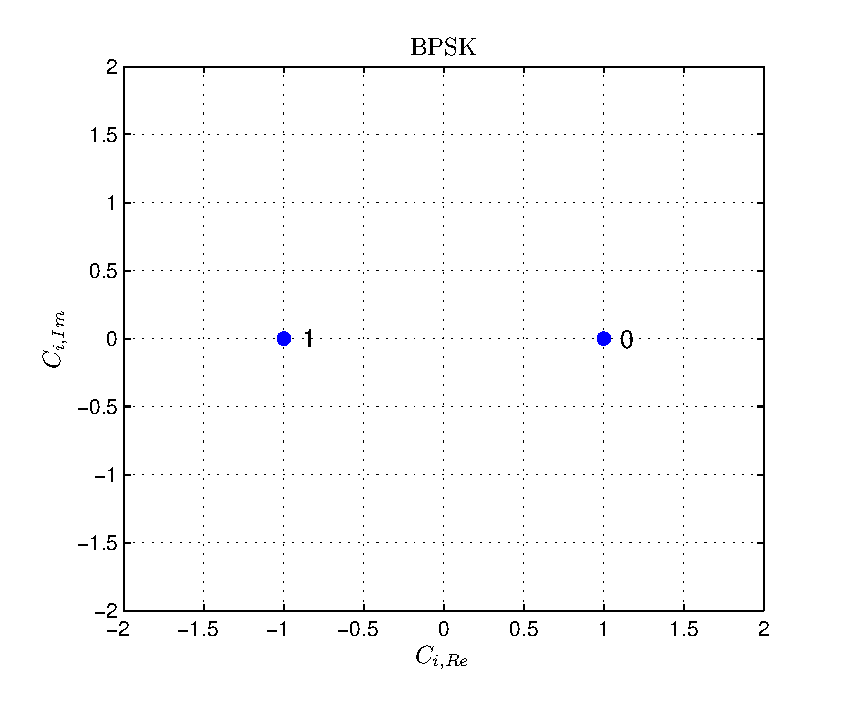
\includegraphics[width=\linewidth]{bpskmapp}
%     \caption{BPSK constellation diagram}\label{fig:BPSK}
%     \end{subfigure}
% \hfill
%     \begin{subfigure}[t]{0.3\textwidth}
%     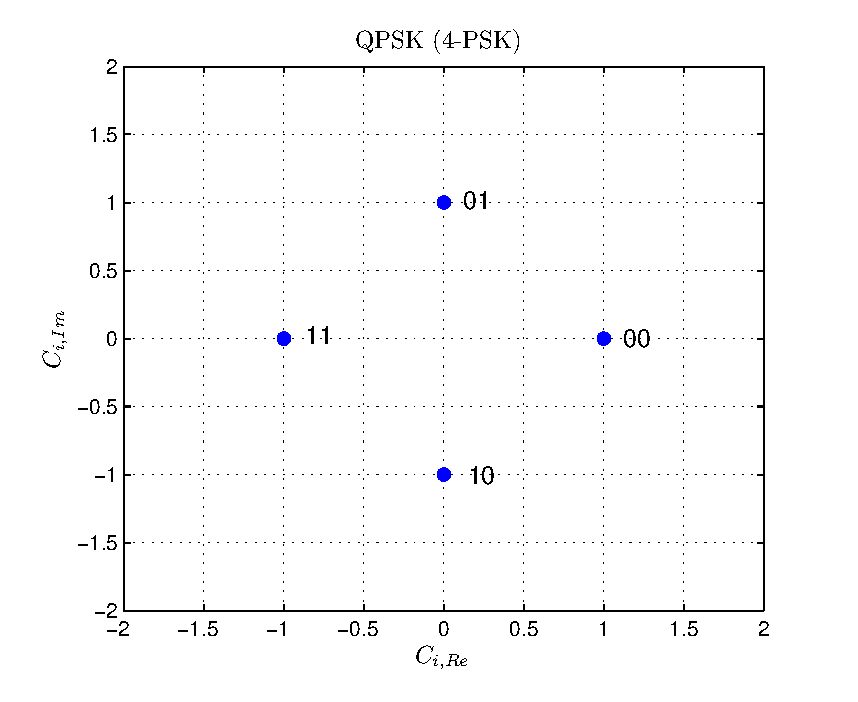
\includegraphics[width=\linewidth]{qpskmapp}
%     \caption{QPSK(4-PSK) constellation diagram}\label{fig:QPSK}
%     \end{subfigure}
% \hfill
%     \begin{subfigure}[t]{0.3\textwidth}
%     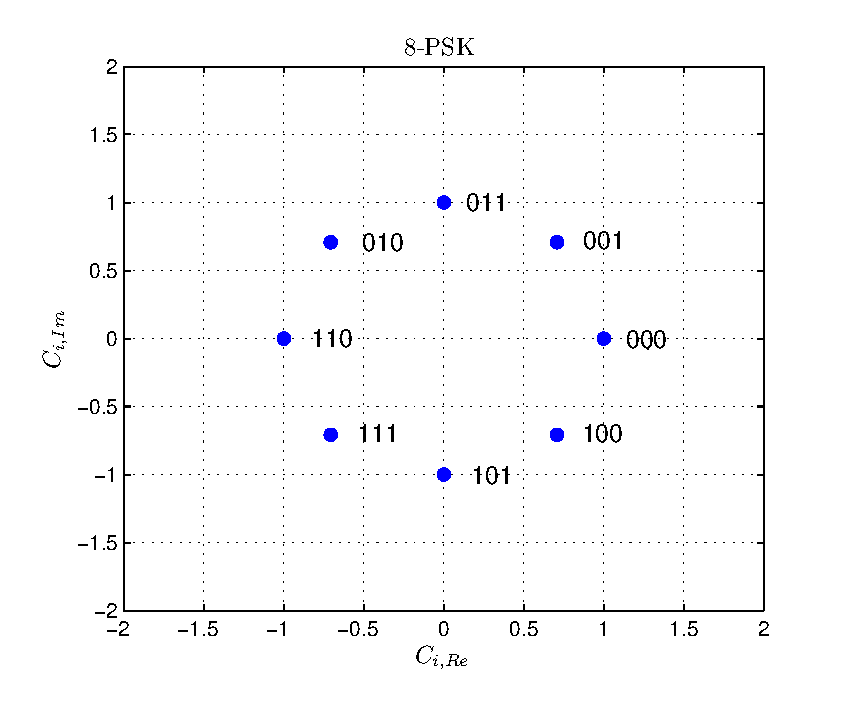
\includegraphics[width=\linewidth]{8pskmapp}
%     \caption{8-PSK constellation diagram}
%     \label{fig:8PSK}
%     \end{subfigure}
% \caption{Gray-coded M-PSK constellation diagrams}
% \label{fig:PSKconstell}
% \end{figure}
%
The simplest \gls{psk} modulation format is \gls{bpsk}, where a logical \glqq 1\grqq\ is encoded as $0$ phase, and a logical \glqq 0\grqq\ is coded as a phase of $\pi$. Then, the modulated symbol, defined in (\ref{eqn:PSKmod}), can be written as
%
\begin{equation}
\label{eqn:BPSKmod}
C_i=\pm \sqrt{S}
\end{equation}
%
with constellation diagram shown in ~\cref{fig:BPSK}. M-\gls{psk} constellation diagram for 4-\gls{psk} ($2$ bits mapped into $4=2^2$ phases) and 8-\gls{psk} ($3$ bits mapped into $8=2^3$ phases), are shown in ~\cref{fig:QPSK} and ~\cref{fig:8PSK}, respectively. Note that they are optimized to minimize the \gls{ber}, resulting in the gray-coded M-PSK constellation, i.e., adjacent constellation points differ in one bit as in ~\cref{fig:PSKconstell}. The BER is defined as the ratio between the number of successfully received to the number of total transmitted information bits and is usually taken as a measure of modulation quality. 

% For \gls{bpsk} in \gls{awgn} it is given as \cite{WiComGoldsmith}
% %
% \begin{equation}
% \label{eqn:BPSKmodBER}
% p_{b,BPSK} = Q\left(\sqrt{\frac{2E_b}{N_0}}\right), 
% \end{equation}
% %
% where $\frac{E_b}{N_0}$ is the SNR\index{SNR} per bit and $Q(x)$ is defined as
% %
% \begin{equation}
% \label{eqn:Qfunction}
% Q(x)=\frac{1}{2}\operatorname{erfc}\left(\frac{x}{\sqrt{2}}\right),
% \end{equation}
% %
% where
% %
% \begin{equation}
% \label{eqn:Erfcfunction}
% \operatorname{erfc}(x)=\frac{2}{\sqrt{\pi}}\int_x^{\infty}{e^{-y^2}dy}
% \end{equation}
% %
% is the complementary error function ($\operatorname{erfc}$).
% For higher order M-\gls{psk}, where $M>4$, the symbol error rate (SER)\index{SER} can be expressed as
% %
% \begin{equation}
% \label{eqn:PSKmodBER}
% p_{s,M-PSK} = 2Q\left( \sqrt{\frac{2E_b\log_2M}{N_0}}\sin{\frac{\pi}{M}}\right),
% \end{equation}
% %
% where 
% \begin{equation*}
% \frac{E_s}{N_0}=\frac{E_b\log_2M}{N_0}
% \end{equation*}
% is the \gls{snr} per symbol. For Gray-coded modulations the \gls{ber} in the high \gls{snr} regime for each modulation is approximately
% \begin{equation*} 
% p_{b,M-PSK} \approx \frac{p_{s,M-PSK}}{\log_2M}.
% \end{equation*}

\subsection{Quadrature Amplitude Modulation (QAM)}
\gls{qam} is a bandwidth efficient signaling scheme that, unlike M-\gls{psk} does not possess a
constant envelope property, thus offering higher bandwidth efficiency, i.e., more bits per second (bps) can be transmitted in a given frequency bandwidth. 






\begin{figure}[hbtp]
    \centering
    \begin{subfigure}[t]{0.3\textwidth}\centering
    \begin{tikzpicture}[x=1.6cm,y=1.6cm]
    % Define the constellation points
    \foreach \i in {0,...,1} {
        \foreach \j in {0,...,1} {
            \pgfmathsetmacro{\x}{-0.5 + \i}
            \pgfmathsetmacro{\y}{-0.5 + \j}
            \node[draw, circle, fill=black, inner sep=0.5pt] at (\x, \y) {};
        }
    }
    % Add axes
    \draw[->] (-1.125,0) -- (1.125,0) node[right] {$I$};
    \draw[->] (0,-1.125) -- (0,1.125) node[above] {$Q$};
    \end{tikzpicture}
    \caption{4-QAM}
    \label{fig:4QAM}
    \end{subfigure}\hfill
    \begin{subfigure}[t]{0.3\textwidth}\centering
        \begin{tikzpicture}[x=0.8cm,y=0.8cm]
    % Define the constellation points
    \foreach \i in {0,...,3} {
        \foreach \j in {0,...,3} {
            \pgfmathsetmacro{\x}{-1.5 + \i}
            \pgfmathsetmacro{\y}{-1.5 + \j}
            \node[draw, circle, fill=black, inner sep=0.5pt] at (\x, \y) {};
        }
    }
    % Add axes
    \draw[->] (-2.25,0) -- (2.25,0) node[right] {$I$};
    \draw[->] (0,-2.25) -- (0,2.25) node[above] {$Q$};
    \end{tikzpicture}
    \caption{16-QAM}
    \label{fig:16QAM}
    \end{subfigure}\hfill
    \begin{subfigure}[t]{0.3\textwidth}\centering
    \begin{tikzpicture}[x=0.4cm,y=0.4cm]
    % Define the constellation points
    \foreach \i in {0,...,7} {
        \foreach \j in {0,...,7} {
            \pgfmathsetmacro{\x}{-3.5 + \i}
            \pgfmathsetmacro{\y}{-3.5 + \j}
            \node[draw, circle, fill=black, inner sep=0.5pt] at (\x, \y) {};
        }
    }
    % Add axes
    \draw[->] (-4.5,0) -- (4.5,0) node[right] {$I$};
    \draw[->] (0,-4.5) -- (0,4.5) node[above] {$Q$};
    \end{tikzpicture}
    \caption{64-QAM}
    \label{fig:64QAM}
    \end{subfigure}
    
    \begin{subfigure}[t]{0.3\textwidth}\centering
    \begin{tikzpicture}[x=0.2cm,y=0.2cm]
        % Define the constellation points
        \foreach \i in {0,...,15} {
            \foreach \j in {0,...,15} {
                \pgfmathsetmacro{\x}{-7.5 + \i}
                \pgfmathsetmacro{\y}{-7.5 + \j}
                \node[draw, circle, fill=black, inner sep=0.5pt] at (\x, \y) {};
            }
        }
        % Add axes
        \draw[->] (-9,0) -- (9,0) node[right] {$I$};
        \draw[->] (0,-9) -- (0,9) node[above] {$Q$};
        \end{tikzpicture}
        \caption{256-QAM}
    \label{fig:256QAM}
    \end{subfigure}\hfill
     \begin{subfigure}[t]{0.3\textwidth}\centering
    \begin{tikzpicture}[x=0.1cm,y=0.1cm]
        % Define the constellation points
        \foreach \i in {0,...,31} {
            \foreach \j in {0,...,31} {
                \pgfmathsetmacro{\x}{-15.5 + \i}
                \pgfmathsetmacro{\y}{-15.5 + \j}
                \node[draw, circle, fill=black, inner sep=0.1pt] at (\x, \y) {};
            }
        }
        % Add axes
        \draw[->] (-18,0) -- (18,0) node[right] {$I$};
        \draw[->] (0,-18) -- (0,18) node[above] {$Q$};
        \end{tikzpicture}
        \caption{1024-QAM}
    \label{fig:1024QAM}
    \end{subfigure}\hfill
     \begin{subfigure}[t]{0.3\textwidth}\centering
    \begin{tikzpicture}[x=0.05cm,y=0.05cm]
        % Define the constellation points
        \foreach \i in {0,...,63} {
            \foreach \j in {0,...,63} {
                \pgfmathsetmacro{\x}{-31.5 + \i}
                \pgfmathsetmacro{\y}{-31.5 + \j}
                \node[draw, circle, fill=black, inner sep=0pt] at (\x, \y) {};
            }
        }
        % Add axes
        \draw[->] (-36,0) -- (36,0) node[right] {$I$};
        \draw[->] (0,-36) -- (0,36) node[above] {$Q$};
        \end{tikzpicture}
        \caption{4096-QAM}
    \label{fig:4096QAM}
    \end{subfigure}
    \caption{QAM constellation diagrams}
\label{fig:QAMconstell}
\end{figure}

\Gls{qam} modulated signals for $M$ constellation points can be written as
%
\begin{equation*}
C_i=\sqrt{S}K(X_i + jY_i),
\end{equation*}
%
where $X_i, Y_i \in \left\lbrace\pm 1, \pm 3,\ldots,\sqrt{M}-1 \right\rbrace$ and $K$ is a scaling factor for normalizing the average power for all constellations to $S$. The $K$ value for various constellations is shown in Table~\ref{tab:param}. Corresponding \gls{qam} constellation diagrams for 4-\gls{qam} ($2$ bits mapped into $4=2^2$ points), 16-\gls{qam} ($4$ bits mapped into $16=2^4$ points), 64-\gls{qam} ($6$ bits mapped into $64=2^6$ points), and 256-\gls{qam} ($8$ bits mapped into $16=2^8$ points), are shown in ~\cref{fig:QAMconstell}. It can be noticed that 4-\gls{qam} corresponds to \gls{qpsk} with constant phase shift $\theta_0 =\pi/4$. 

\Gls{qam} schemes are used in several typical wireless digital communications specifications for a long time. A trend is the drastic increase in modulation depth as can be seen in \cref{tab:wifi-qam}.


% \begin{figure}[thb]
% \centering

% \begin{subfigure}[b]{0.42\textwidth}
%     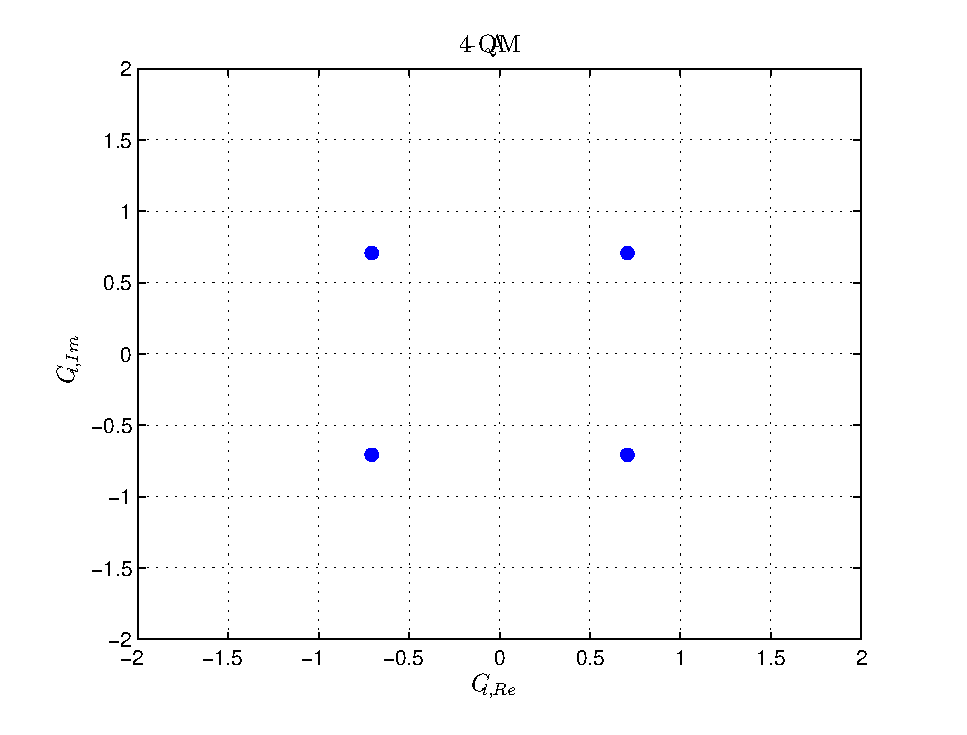
\includegraphics[width=\linewidth]{figs/4-QAM.eps}
%     \caption{4-QAM constellation diagram}
%     \label{fig:4QAM}
%     \end{subfigure}%
% \begin{subfigure}[b]{0.42\textwidth}
%     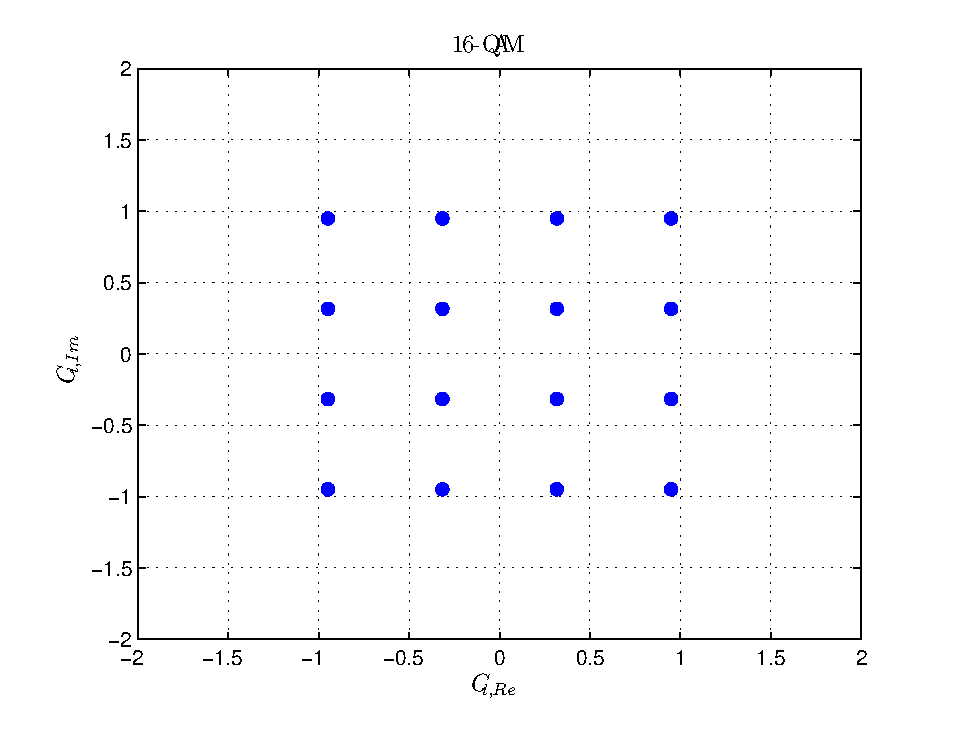
\includegraphics[width=\linewidth]{figs/16-QAM.eps}
%     \caption{16-QAM constellation diagram}
%     \label{fig:16QAM}
%     \end{subfigure}

% \begin{subfigure}[b]{0.42\textwidth}
%     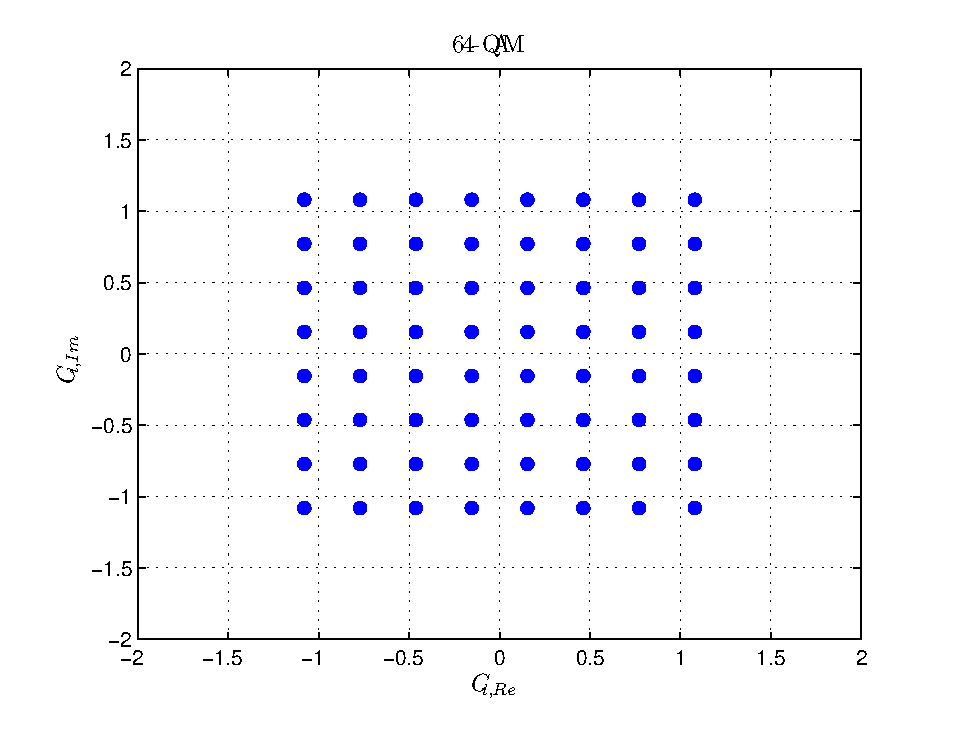
\includegraphics[width=\linewidth]{figs/64-QAM.eps}
%     \caption{64-QAM constellation diagram}
%     \label{fig:64QAM}
%     \end{subfigure}%
% \begin{subfigure}[b]{0.42\textwidth}
%     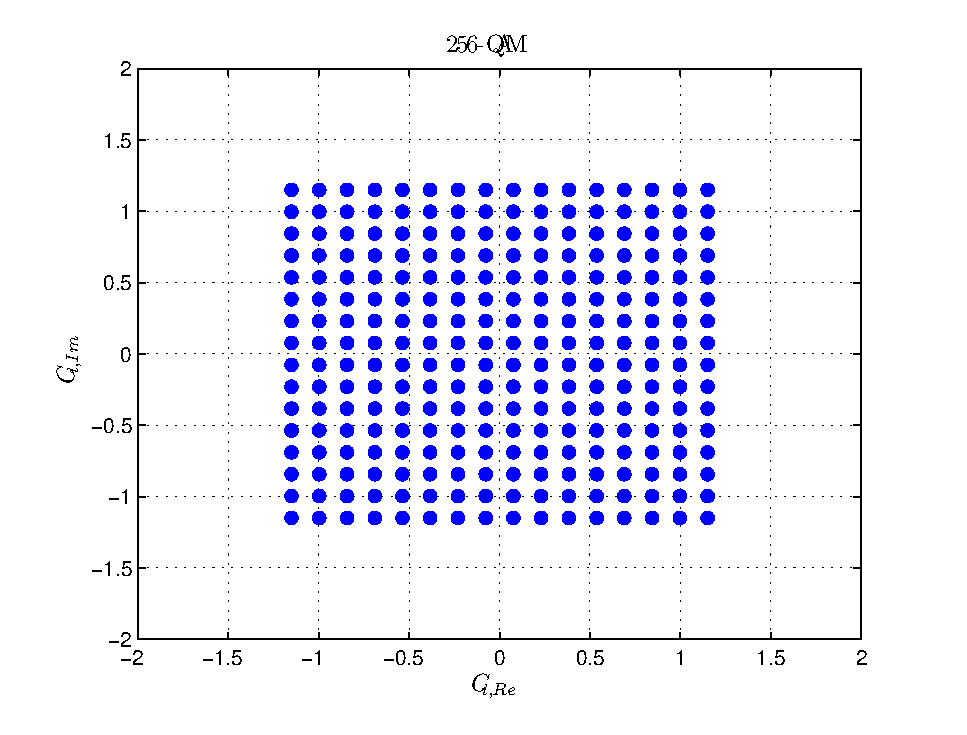
\includegraphics[width=\linewidth]{figs/256-QAM.eps}
%     \caption{256-QAM constellation diagram}
%     \label{fig:256QAM}
%     \end{subfigure}
% %%\end{center}
% \caption{QAM constellation diagrams}
% \label{fig:QAMconstell}
% \end{figure}
%

%
\begin{table}[htb]
\centering
\scriptsize
\renewcommand\arraystretch{1.6}
\caption{Modulation dependent parameters}\label{tab:param}
\begin{tabular}{ p{3cm} p{3cm} p{3cm}}\toprule
Modulation&Number of bits $m$&$K$\\\midrule
4-QAM&2&$1/\sqrt{2}$\\
16-QAM&4&$1/\sqrt{10}$\\
64-QAM&6&$1/\sqrt{42}$\\
256-QAM&8&$1/\sqrt{170}$\\\bottomrule
\end{tabular}
\end{table}
%
% The \gls{ser} for \gls{qam} modulations can be expressed as
% %
% \begin{equation*}
% %\label{eqn:MQAMmodSER}
% p_{s,M-QAM} = 1-\left( 1-2\left( 1-\frac{1}{\sqrt{M}}\right)Q\left( \sqrt{3\frac{E_b\log_2 M}{(M-1)N_0}}\right) \right) ^2.
% \end{equation*}
% %
% where $Q(x)$ is defined in (\ref{eqn:Qfunction}). For Gray-coded modulations  the \gls{ber} in the high \gls{snr} regime for each modulation is, as for M-PSK case, approximately
% \begin{equation}
% \label{eqn:MQAMmodBER}
% p_{b,M-QAM} \approx \frac{p_{s,M-QAM}}{\log_2M}.
% \end{equation}


\begin{table}[hbtp]
    \centering
    \scriptsize
    \caption{Overview of maximum modulation depth in Wi-Fi.~\cite{enwiki:1210657347}}
    \label{tab:wifi-qam}
\renewcommand\arraystretch{1.6}
    \begin{tabular}{l l l r}
    \toprule
    Wi-Fi standard & IEEE standard & Modulation Depth & bits per symbol\\
    \midrule
    Wi-Fi 5 & 802.11ac   &  256-QAM& 8\\
    Wi-Fi 6(E) & 802.11ax   &  1024-QAM & 10\\
    Wi-Fi 7 & 802.11be   &  4096-QAM &12\\
    Wi-Fi 8 & 802.11bn   &  8192-QAM &13\\
    \bottomrule
    \end{tabular}
    
\end{table}


\chapter{Software Defined Radio and GNU Radio Framework}\label{sec:sdrgnur}

In this chapter a general introduction to the \gls{sdr} concept is given. Additionally, advantages of SDRs and given hardware limitations are addressed. Here, the GNU Radio SDR framework is presented giving insight into the basic architectural features.

An \gls{sdr} is a radio that is built entirely or in large parts in software, which runs on a general purpose computer. A more extensive definition is given by Joseph Mitola, who established the term Software Radio~\cite{Mitola200609}:

\say{A software radio is a radio whose channel modulation waveforms are defined in software. That is, waveforms are generated as sampled digital signals, converted from digital to analog via a wideband \gls{dac} and then possibly upconverted from \gls{if} to \gls{rf}. The receiver, similarly, employs a wideband \gls{adc} that captures all of the channels of the software radio node. The receiver then extracts, downconverts and demodulates the channel waveform using software on a general purpose processor. Software radios employ a combination of techniques that include multi-band antennas and \gls{rf} conversion; wideband \gls{adc} and \gls{dac}; and the implementation of \gls{if}, baseband and bitstream processing functions in general purpose programmable processors. The resulting software defined radio (or software radio) in part extends the evolution of programmable hardware, increasing flexibility via increased programmability.}


This means, that instead of using analog circuits or a specialized \gls{dsp} to process radio signals, the digitized signals are processed by architecture independent, and high level software running on general purpose processors. The term radio designates any device, that transmits and/or receives radio waves. While most modern radios contain firmware that is written in some kind of programming language, the important distinction in a software radio is that it is not tailored to a specific chip or platform, and it is therefore possible to reuse its code across different underlying architectures~\cite{DABETH}.

\section{Ideal Software Defined Radio and Practical Limitations}\label{sec:sdr}

In the ideal case, the only hardware that is needed besides a computer is an antenna and an \gls{adc} for the receiver, as well as a \gls{dac} for the transmitter. An \gls{sdr} would thus look as depicted in {~\cref{fig:idealsdr}}. In the receiver, a transmitted radio signal is picked up by an antenna, and then fed into an \gls{adc} to sample it. Once digitized, the signal is sent to some general purpose computer (e.g. an embedded PC) for processing. The transmitter looks very similar, except that the signal is sent in the reverse direction, and a \gls{dac} is used instead of an \gls{adc}. In a complete transceiver, the processing unit and the antenna may be shared between receiver and transmitter.

While the approach presented in the previous section is very simple and (in the ideal case) extremely versatile, it is not practical, due to limitations in real hardware. However, various solutions have been suggested to overcome these problems. A quick look at the different hardware limitations is given below. For better readability, only the receiving side is discussed. The transmitting side is constructed symmetrically.
%
\begin{figure}[thb]
\centering
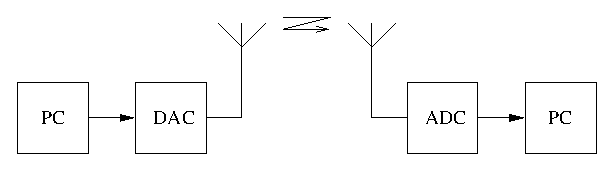
\includegraphics[width=0.6\linewidth]{idealsdr.eps}
\caption{Ideal SDR transmission\label{fig:idealsdr}}
\end{figure}
%
\begin{itemize}
 \item \textit{\Acrlong{adc}}: According to the Nyquist sampling theorem, the sampling rate of the \glspl{adc}  must be at least twice as high as the bandwidth of received signal which limits the maximum bandwidth of the received signal. Conventional \glspl{adc} are capable of sampling rates in the area of \SI{500}{Msps}, which translates to a bandwidth of \SI{250}{\mega\hertz}. While this bandwidth is enough for most current applications, the carrier frequency is usually higher than \SI{250}{\mega\hertz}. In practice, a \gls{rf} frontend is therefore usually required, to convert the received signal to an \gls{if}. Notably, as of 2018 there exists 12-bit \glspl{adc} which can sample at \SI{6.4}{\giga s\per\second}. This allows to directly digitize\footnote{Therefore it is often called direct-RF sampling.} signals at \gls{rf} frequencies and achieve sufficient dynamic range for modern communications. However, this technology is costly and not energy-efficient.
 
The second parameter, the \gls{adc} resolution influences the dynamic range of the receiver. As each additional bit doubles the resolution of the sampled input voltage, the dynamic range can be roughly estimated as $R = 6dB \times n$ where $R$ is the dynamic range and $n$ the number of bits in the \gls{adc}. As \glspl{adc} used for \gls{sdr} usually have a resolution of less than 16 bits, it is important to filter out strong interfering signals, such as signals from mobile phones, before the wideband \glspl{adc}. This is usually done in the \gls{rf} frontend. 

\item \textit{Bus Speed}: Another problem lies in getting the data from the \gls{adc} to the computer. For any practical bus, there is a maximum for the possible data rate, limiting the product of sample rate and resolution of the samples. The speed of common buses in commodity PCs ranges from a few Mbps to several Gbps as an example, the \gls{pcie} Gen~5 bus has a theoretical maximum speed of \SI{64}{\giga\byte\per\second} (in one direction). However, the speed is limited by the connections on your PC. For USB-C has a theoretical transfer speed of \SI{20}{\giga\bit\per\second}, which would not support transfering direct-\gls{rf} samples. 

\item \textit{Performance of the Processing Unit}: For real-time processing, the performance of the \gls{cpu} and the sample rate limit the number of mathematical operations that can be performed per sample, as samples must be processed as fast as they arrive. In practice, this means that fast \glspl{cpu}, clever programming and possibly parallelization is needed. If this does not suffice, a compromise must be found, to use a less optimal but faster signal processing algorithm.

\item \textit{Latency}: Since general purpose computers are not designed for real-time applications, a rather high latency can occur in practical \glspl{sdr}. While latency is not much of an issue in transmit-only or receive-only applications, many wireless standards, such as \gls{lte} require precise timing, and are therefore very difficult to implement in an \gls{sdr}.
\end{itemize}

Hence, we need to reduce the number of samples. This is done by first down-converting the analog \gls{rf} signal to an \acrlong{if} (superheterofyne receiver) or directly to baseband and perform quadrature sampling  (direct conversion or zero-IF). 

\begin{figure}[hbtp]
    \centering
    \begin{subfigure}[b]{0.32\textwidth}
         \centering
         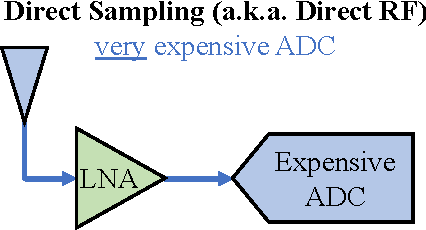
\includegraphics[width=0.9\textwidth]{figs/direct-rf.pdf}
         \caption{Direct RF}
         \label{fig:direct-rf}
     \end{subfigure}
     \hfill
     \begin{subfigure}[b]{0.32\textwidth}
         \centering
         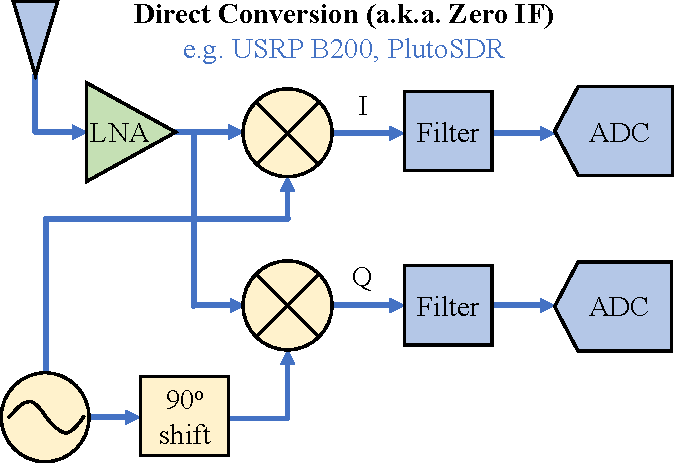
\includegraphics[width=0.9\textwidth]{figs/zero-if.pdf}
         \caption{Zero IF}
         \label{fig:zero-if}
     \end{subfigure}
     \hfill
     \begin{subfigure}[b]{0.32\textwidth}
         \centering
         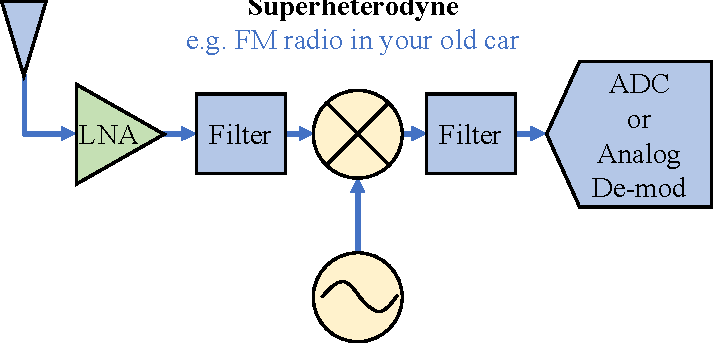
\includegraphics[width=0.9\textwidth]{figs/superheterodyne.pdf}
         \caption{Superheterodyne}
         \label{fig:superheterodyne}
     \end{subfigure}
    \caption{RF Architectures (from \url{pysdr.org})}
    \label{fig:rf-arch}
\end{figure}

Because of the use of general purpose processing units, an implementation of a given wireless
application as an \gls{sdr} is likely to use more power and occupy more space than a hardware radio
with analog filtering and possibly a dedicated signal processor. Because an \gls{sdr} contains more
complex components than a hardware radio, it will likely be more expensive, given a large
enough production volume.

Nevertheless, \gls{sdr} concepts carry the flexibility of software over to the radio world and introduces a number of interesting possibilities.
For example, very much the same way as someone may load an alternative word processor or Internet
browser on a PC, depending on the task at hand, a \gls{sdr} could allow its user to load a different
configuration, depending on whether the user wants to listen to a broadcast radio transmission,
place a phone call or determine the position via \gls{gps}.%A new
%application may even be added after the device is finished. 
Since the same hardware can be used
for any application, a great reuse of resources is possible. Another interesting possibility enabled by \gls{sdr} is the creation of a cognitive radio, which is
aware of its \gls{rf} environment and adapts itself to changes in the environment. By doing this,
a cognitive radio can use both the \gls{rf} spectrum and its own energy resources more efficiently.
As a cognitive radio requires a very high degree of flexibility, the concept of \gls{sdr} is very convenient for its practical realization.

\section{GNU Radio Architecture}\label{sec:gnur}

GNU~Radio is an open source, free software toolkit for building \glspl{sdr} \cite{GNUR}. It is designed to run on commodity computers combined with minimal hardware, allowing the construction of simple software radios \cite{DABETH}. The project was started in early 2000 by Eric Blossom and has evolved into a mature software infrastructure that is used by a large community of developers. It is licensed under the \gls{gpl}, thus anyone is allowed to use, copy and modify GNU~Radio without limits, provided that extensions are made available under the same license. While GNU~Radio was initially started on a Linux platform, it now supports various Windows, MAC and various Unix platforms.

GNU~Radio architecture consists of two components. The first component is the set of numerous building blocks which represents \Cpp\ implementations of digital signal processing routines such as (de)modulation, filtering, (de)coding and I/O operations such as file access, for further information about \Cpp\ programming see for example~\cite{Meyers,Meyers2,Meyers3,Stroustrup,Sutter}. The second component is a framework to control the data flow among blocks, implemented as Python scripts enabling easy reconfiguration and control of various system functionalities and parameters, for further studies on Python see e.g.,~\cite{Martelli}. By \textit{wiring} together such building blocks, a user can create a software defined radio, similar to connecting physical \gls{rf} building blocks to create a hardware radio. An \gls{rf} interface for GNU~Radio architecture is realized by \gls{usrp} boards, a general purpose \gls{rf} hardware, which performs computationally intensive operations as filtering, up- and down-conversion. The \gls{usrp} B210s connected via USB, which we will be using in this lab, are controlled through a robust \gls{api} provided by GNU~Radio.\footnote{Note that the \glspl{usrp} can also be programmed with the UHD library from Ettus. This provides a more low-level access to the device, and is therefore out of scope of this lab.}
\subsection{Gnu Radio Framework}
A data flow among different blocks is abstracted by \textbf{flowgraph}, a directed acyclic graph in which the vertices are the GNU~Radio blocks and the edges corresponds to data \textbf{streams}, as shown in ~\cref{flowgraph}. 
%
\begin{figure}[thb]
\centering
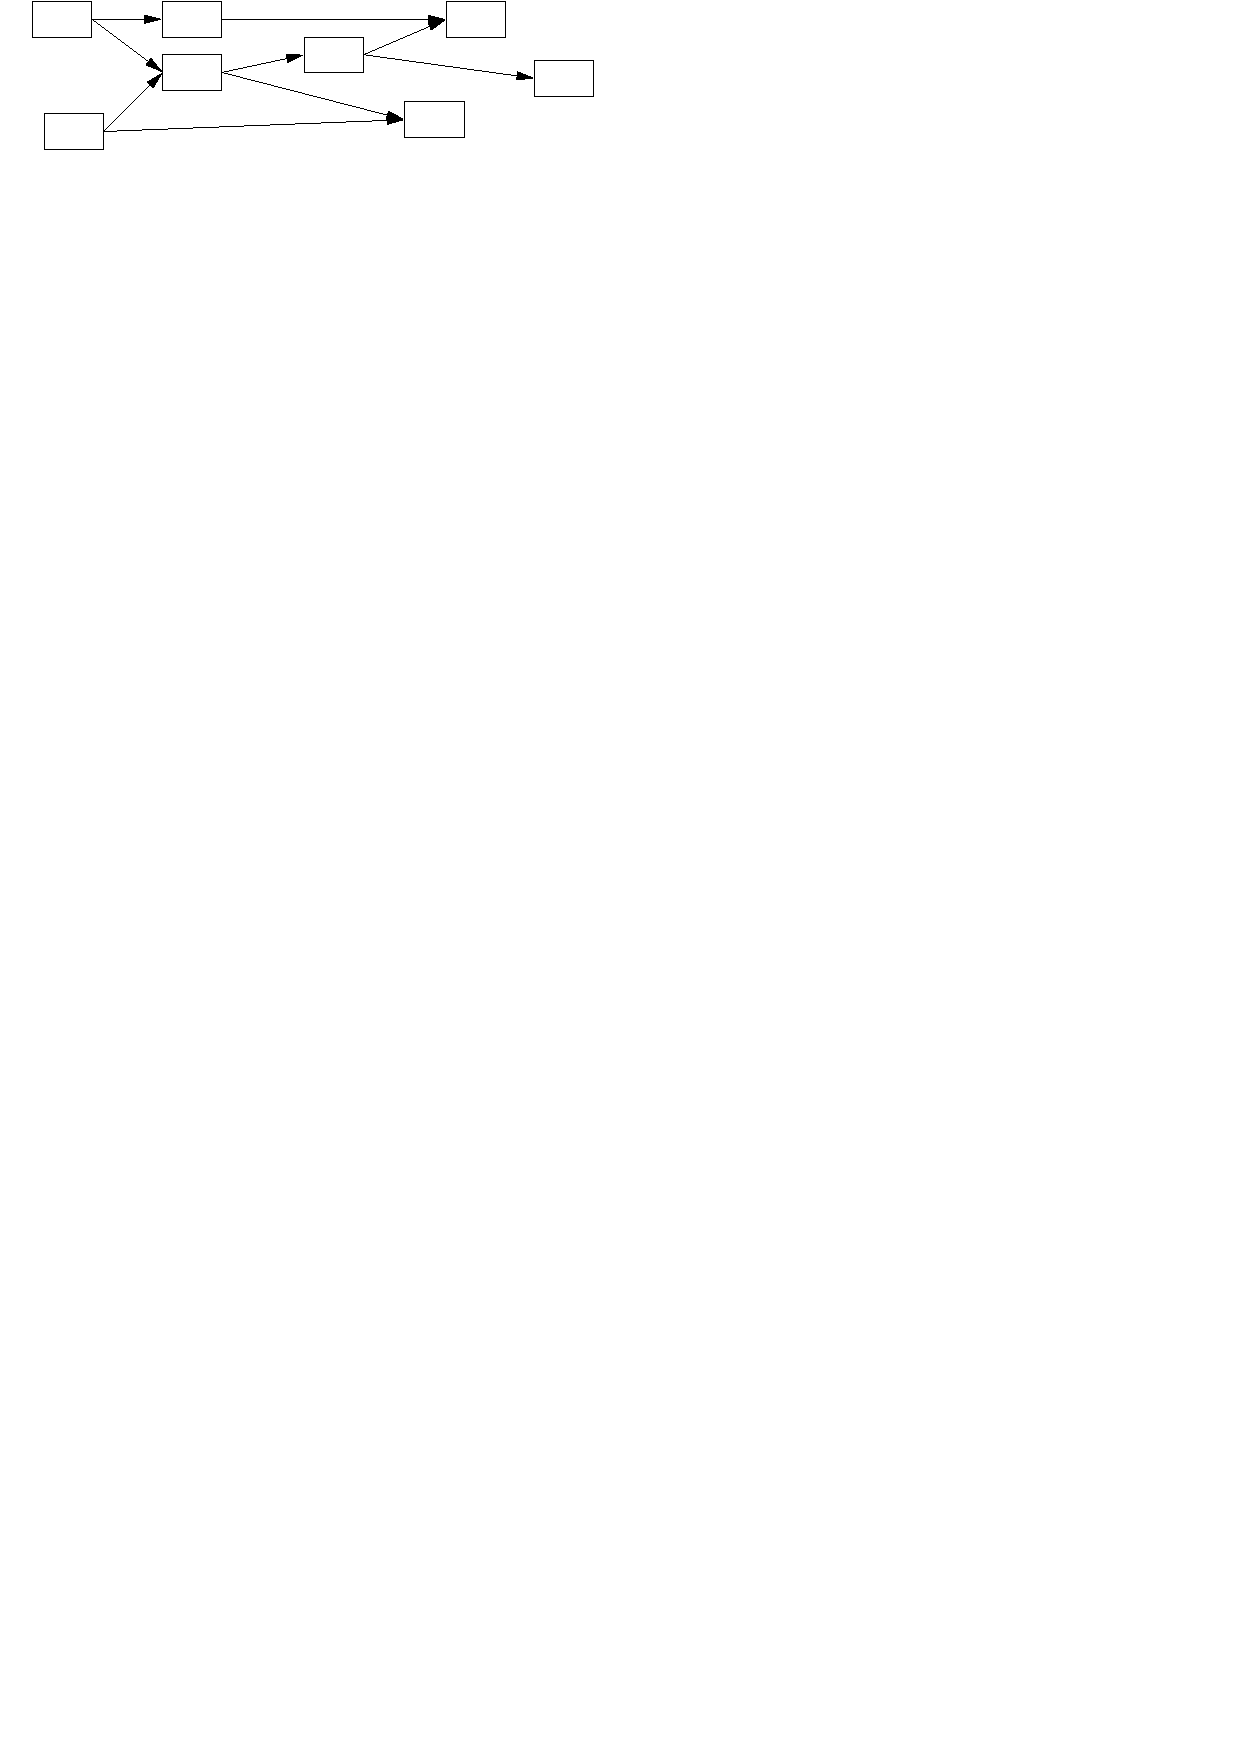
\includegraphics{gr_graph_example}
\caption{An example of \textbf{flowgraph}}\label{flowgraph}
\end{figure}
%
Generally, GNU~Radio blocks, shown in ~\cref{fig:gnuradio_block} operate on continuous streams of data. Most blocks have a set of input and/or output ports, therefore, they consume data from input streams and generate data for their output streams. Special blocks called sources and sinks only consume or produce data, respectively. Examples of sources and sinks are blocks that read and write, respectively, from \gls{usrp} receive ports, sockets, and file descriptors. Each block has an input and output signature (IO signatures) that defines the minimum and maximum number of input and output streams it can have, as well as the size of the data type on the corresponding stream. Examples of supported types are
\begin{itemize}
 \item \texttt{c} - complex interleaved floats (8 byte each),
\item \texttt{f} - floats (4 byte),
\item \texttt{s} - short integers (2 byte) and
\item \texttt{b} - byte integers (1 byte).
\end{itemize}
%
\begin{figure}[thb]
\centering
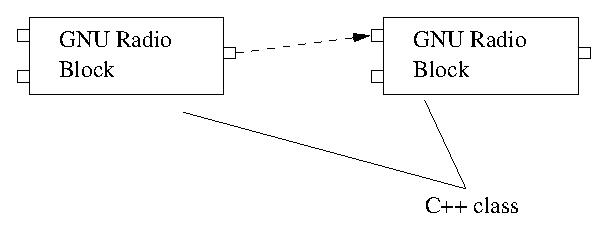
\includegraphics{gr_blocks.eps}
\caption{GNU Radio blocks}\label{fig:gnuradio_block}
\end{figure}

A full list of the supported data types can be found in GNU Radio Companion by clicking on \texttt{Help~>~Types}.
%

Each block defines a \textbf{general\_work()} function that operates on its input to produce output streams. In order to help the scheduler decide when to call the work function, blocks also provide a \textbf{forecast()} function that returns the system runtime, the number of input items it requires to produce a number of output items and how many output items it can produce given a number of input items. At runtime, blocks tell the system how many input (output) items they consumed (produced). Blocks may consume data on each input stream at a different rate, but all output streams must produce data at the same rate. The input and output streams of a block have buffers associated with them. Each input stream has a read buffer, from which the block reads data for processing. Similarly, after processing, blocks write data to the appropriate write buffers of its output streams. The data buffers are used to implement the edges in the flowgraph: the input buffers for a block are the output buffers of the upstream block in the flowgraph. GNU~Radio buffers are single writer, multiple reader FIFO (First in First Out) buffers.
%
\begin{figure}[thb]
\centering
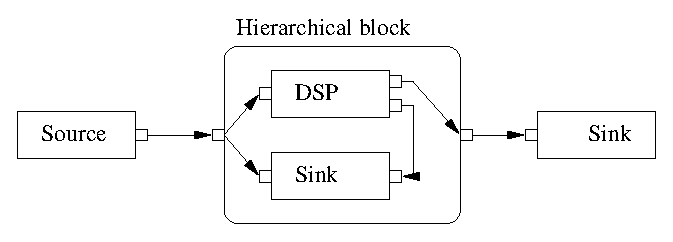
\includegraphics{hier_flowgraph.eps}
\caption{An example of a flowgraph with a hierarchical block}\label{fig:hier_flowgraph}
\end{figure}
%
Several blocks are connected in Python\index{Python} forming a flowgraph using the \textbf{connect} function which specifies how the output stream(s) of a processing block connects to the input stream of one or more downstream blocks. The flowgraph mechanism then automatically builds the flowgraph; the details of this process are hidden from the user. A key function during flowgraph construction is the allocation of data buffers to connect neighboring blocks. The buffer allocation algorithm considers the input and output block sizes used by blocks and the relative rate at which blocks consume and produce items on their input and output streams. Once buffers have been allocated, they are connected with the input and output streams of the appropriate block.

Several blocks can also be combined in a new block, named \textbf{hierarchical} block, as shown in ~\cref{fig:hier_flowgraph}. \textbf{Hierarchical} blocks are implemented in Python and together with other blocks can be combined into new \textbf{hierarchical} blocks. Input and output ports of hierarchical blocks have same constraints as those of terminal blocks.

The GNU~Radio scheduler executes the graph that was built by the flowgraph mechanism. During the execution, the scheduler queries each block for its input requirements and it uses the above-mentioned forecast functions to determine how much data the block can consume from its available input. If sufficient data is available in the input buffers, the scheduler calls the block's work function. If a block does not have sufficient input, the scheduler simply moves on to the next block in the graph. Skipped blocks will be executed later, when more input data is available. The scheduler is designed to operate on continuous data streams.
%
\begin{figure}[thb]
\centering
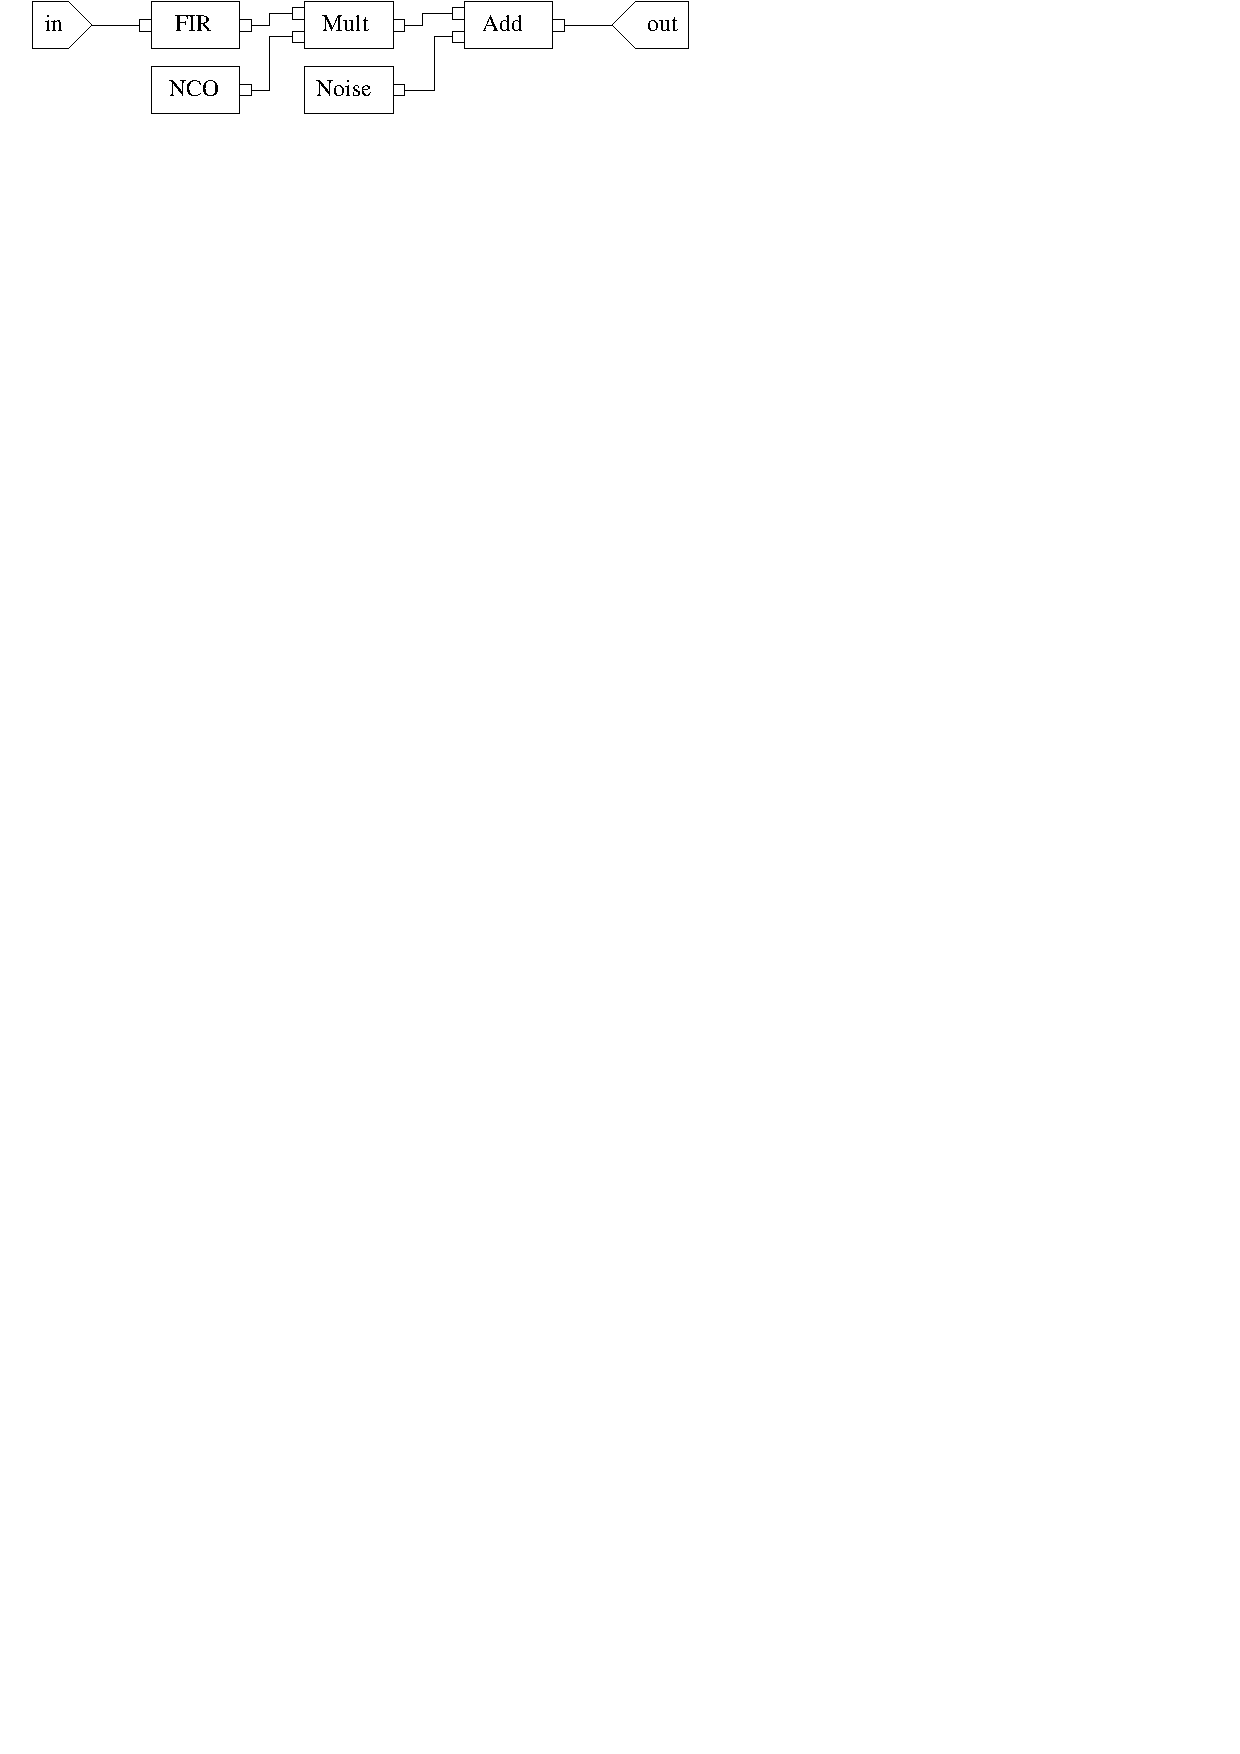
\includegraphics{gralg_example}
\caption{Wireless communication channel simulation model}\label{fig:gralg_example}
\end{figure}

\subsection{An Example: Wireless Channel Simulation}

It will be shown how a model for a static wireless channel can be implemented as a GNU~Radio \textbf{hierarchical} block. The channel is affected by multipath propagation, frequency offset and additive noise. ~\cref{fig:gralg_example} shows a model with internal blocks and corresponding ports \cite{Auras}.

Multipath effects are modeled using a FIR-filter where complex filter coefficients are taken from an arbitrary channel model, e.g., Rayleigh channel model. The signal from an input port is derived to the corresponding GNU~Radio block \textbf{gr.fir\_filter\_ccc}. The suffix ccc denotes that the input stream, output stream and filter coefficients are of complex data types.

According to (\ref{eqn:received_time_freqshift}), the frequency offset is modeled as a sinus wave with fixed frequency and is multiplied with the incoming signal. The corresponding GNU radio blocks are the complex sine signal source \textbf{gr.sig\_source\_c} and the multiplicator with complex inputs and outputs \textbf{gr.multiply\_cc}, respectively.

Finally, complex additive Gaussian noise generated by \textbf{gr.noise\_source\_c} is added to the incoming signal in the \textbf{gr.add\_cc} block and the result is directed to the output port.

The initial parameters of a given hierarchical block, named \textbf{simple\_channel}, are additive noise standard variance, frequency offset normalized to sampling frequency and complex FIR-filter coefficients. IO signatures of input and output ports are identical, and in the framework there is minimum one port and maximum one port for both input and output.

During runtime, internal blocks are initialized and connected to the flowgraph.
The corresponding python\index{Python} script is shown below.
\begin{program}[thb]
\begin{verbatim}
class simple_channel(gr.hier_block2):
  def __init__(self, noise_rms, frequency_offset, channel_coefficients):
    gr.hier_block2.__init__(self, "simple_channel", # Blocktype Identifier
        gr.io_signature(1,1,gr.sizeof_gr_complex),  # incoming
        gr.io_signature(1,1,gr.sizeof_gr_complex))  # outgoing

    # for example channel_coefficients = [0.5+0.1j, 0.2-0.01j]
    multipath_sim = gr.fir_filter_ccc(1, channel_coefficients)

    # frequency_offset normalized to sampling frequency
    # amplitude = 1.0, DC offset = 0.0
    offset_src = gr.sig_source_c(1, gr.GR_SIN_WAVE, frequency_offset, 1.0, 0.0)
    mix = gr.multiply_cc()

    # noise_rms -> var(noise) = noise_rms**2
    noise_src = gr.noise_source_c(gr.GR_GAUSSIAN, noise_rms/sqrt(2))
    add_noise = gr.add_cc()

    # describe signal paths
    self.connect(self, multipath_sim)       # incoming port
    self.connect(multipath_sim, (mix,0))
    self.connect(offset_src, (mix,1))
    self.connect(mix, (noise_add,0))
    self.connect(noise_src, (noise_add,1))
    self.connect(noise_add, self)           # outgoing port
\end{verbatim}
\caption{Python script for simulation of a wireless communication channel}
\end{program}

\section{Installing GNU Radio}

GNU Radio can be run on multiple \glspl{os}, although the most reliable platform is a Linux-based environment, e.g., Ubuntu or Mint.
For Windows and macOS Radioconda can be installed, which bundles a collection of cross-platform installers for numerous open-source software radio packages.

More instructions can be found at \url{https://wiki.gnuradio.org/index.php?title=InstallingGR}. \textbf{Do not} follow the instructions under \textit{Other Installation Methods}. If not clear, contact your lab assistant.







%\chapter{GNU Radio OFDM Transceiver Implementation}\label{sec:TIOFDM}%
%
This chapter gives an introduction to an \gls{sdr} based GNU Radio OFDM transceiver implemented in our institute \cite{MZDARM}.
%
\begin{figure}[thb]
\centering
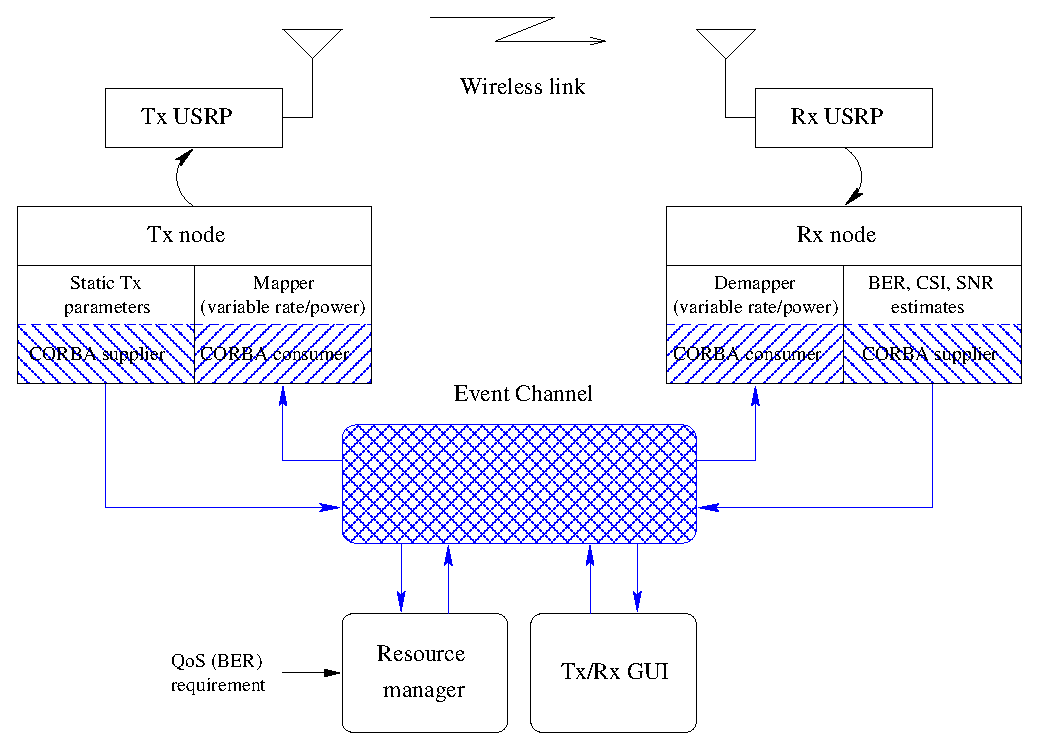
\includegraphics[width=0.54\linewidth]{grp_04.eps}
\caption{System overview\label{fig:sys_dig}}
\end{figure}
%
A system diagram of our \gls{ofdm} framework is shown in~\cref{fig:sys_dig}. Transmitter and receiver nodes are composed of a host commodity computer and general purpose \gls{rf} hardware, \gls{usrp}. The baseband signal processing at the host computers is implemented in the GNU~Radio framework.
%
\begin{figure}[ht]
\centering

 \begin{subfigure}[b]{0.56\linewidth}
 \centering
 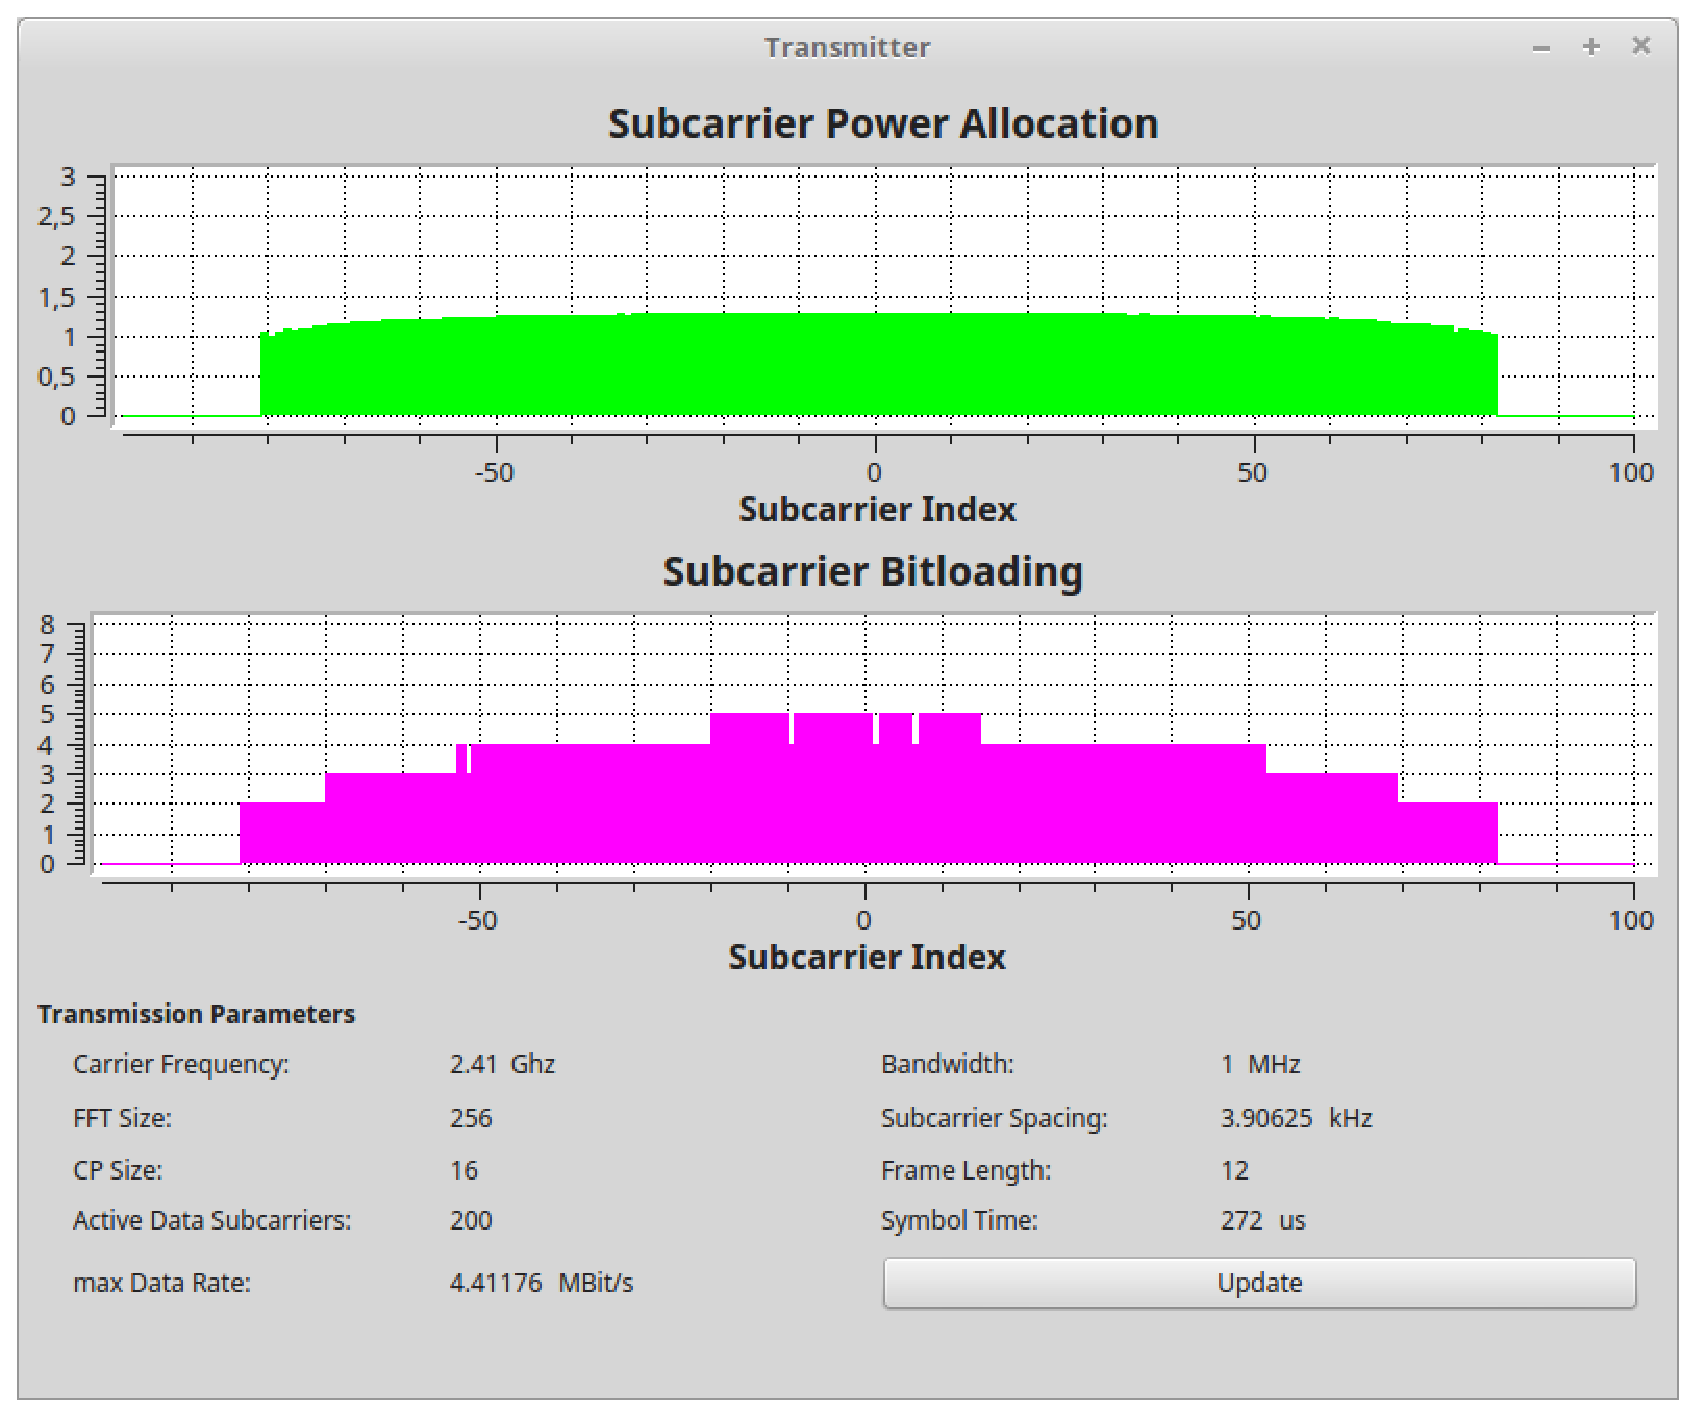
\includegraphics[width=\textwidth]{screenshot_tx.eps}
 \caption{The transmitter's GUI}\label{fig:txgui}
 \end{subfigure}

 \begin{subfigure}[b]{0.56\linewidth}
 \centering
 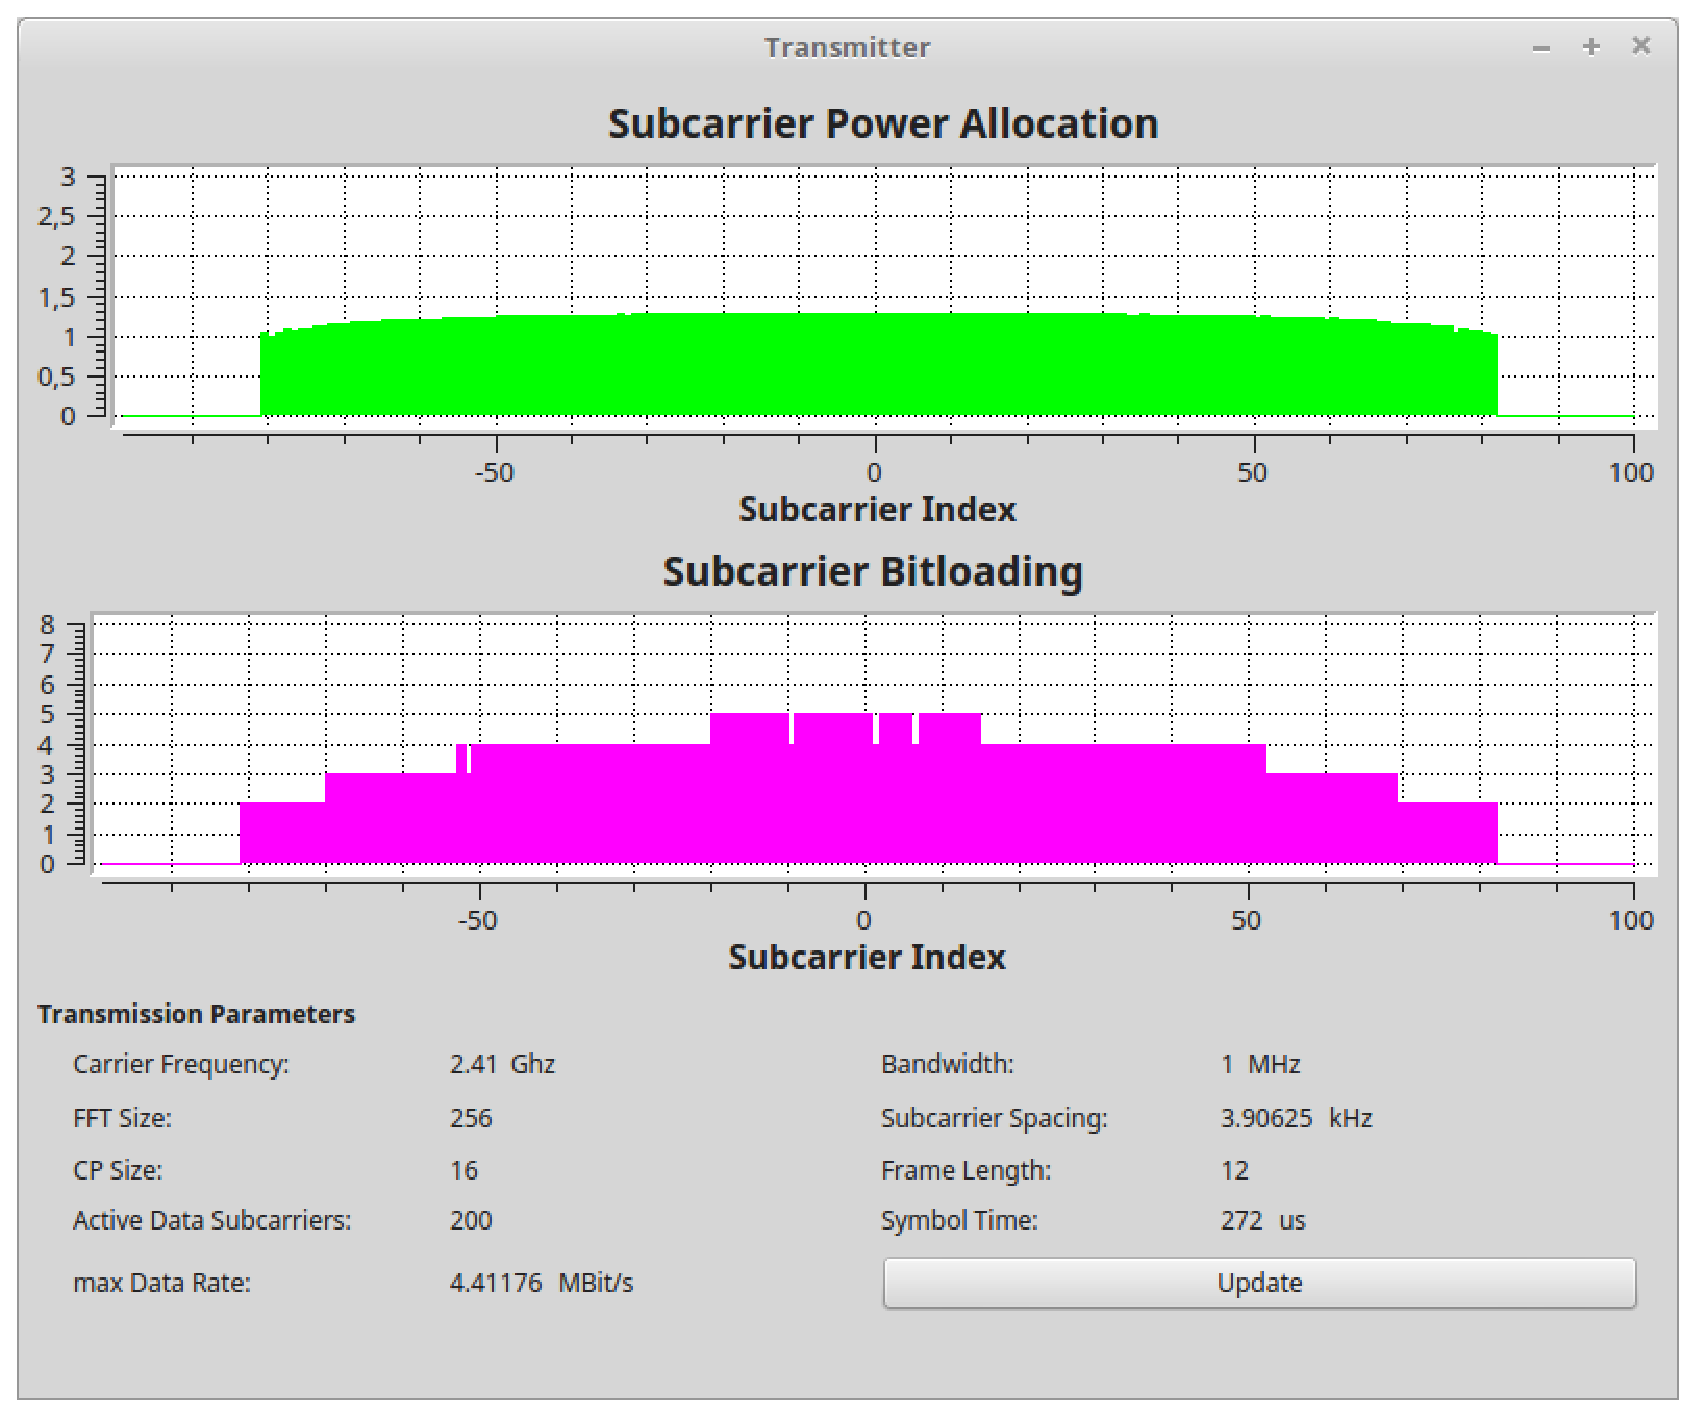
\includegraphics[width=0.665\linewidth]{screenshot_tx.eps}
 \caption{The receiver's GUI with interactive control interface}\label{fig:rxgui}
 \end{subfigure}
\caption{The framework's GUI with interactive control interface\label{fig:txrxgui}}
\end{figure}%
%
Within the framework, additional \gls{ofdm} specific GNU~Radio blocks are implemented, particularly at receiver's synchronization stage, since \gls{ofdm} systems are highly sensitive to \gls{to} and oscillators' mismatch between transmitter and receiver due to necessity for subchannel orthogonality, see Section~\ref{sec:sysimp}. The main adaptive and capacity achieving functionality is performed in blocks for adaptive mapping and demapping of various rates (taken from the set of available modulations given in Table~\ref{tab:tabtab}.1) and power levels across subchannels.
%
\begin{table}[tb]
\label{tab:tabtab}
\centering
{\scriptsize\begin{tabular}{| p{4.5cm}| p{5.5cm}|}\hline
Carrier frequency (\textbf{static})&$2400-2483$ MHz\\\hline
Bandwidth (\textbf{static})& Variable, up to $2$ MHz\\\hline
FFT length (\textbf{static})& $64-1024$\\\hline
Frame length (\textbf{static}) & Variable \\\hline
Modulations (\textbf{dynamic})&BPSK, QPSK, 8-PSK, 16-QAM, 32-QAM, 64-QAM, 128-QAM, 256-QAM\\\hline
Power (\textbf{dynamic})& Up to 20 mW\\\hline
\end{tabular} }%
\caption{OFDM symbol parameters}%
\end{table}%
%
Algorithms for estimation of link quality, expressed through average \gls{snr} and \gls{csi} over subchannels, are extensively studied and implemented at the receiver. Furthermore, in order to assess system performance, the receiver implementation contains blocks for \gls{ber} measurements.

The communication between transmitter and receiver node is organized as a reconfigurable continuous one-way transmission of OFDM symbol frames. As shown in Table~\ref{tab:tabtab}.1, the set of input configuration parameters can be divided into two classes. The set of \textbf{static parameters} containing \gls{fft}, number of subchannels, frame size, etc., is initialized at transmission start and is known to both nodes. The set of \textbf{dynamic parameters} which are reconfigurable at runtime includes total transmit power and allocated rate and power over subchannels.

The backbone of the system is realized over a local Ethernet network by a \CORBA\index{CORBA} \textbf{event service}~\cite{GNUCORBA}, a distributed communication model that allows an application to send an event that will be received by any number of objects located in different logical and/or physical entities, for more information on CORBA see~\cite{Mowbray,Orfali}. Estimated parameters that indicate link quality (average \gls{snr}, \gls{csi}, and \gls{ber}) and current static transmitter's parameters are supplied as \CORBA\index{CORBA} events to the \textbf{event channel} which allows other components (consumers) within the system to register their interests in events. The central control unit that determines optimal input transmission parameters for given requirements is called \textbf{resource manager}. Controlled by an interactive \gls{gui}\ it consumes supplied events forwarded from the \textbf{event channel}, performs allocation in an optimal manner, and supplies new transmission parameters, i.e., total transmit power and power/rate per subchannel, which are finally consumed by other components in the system.

The \GUI, facilitating the demonstration, is developed in Qt/\Cpp\ framework. The transmitter's \gls{gui} contains static transmission parameters and current allocation of rate and power over subchannels, as shown in ~\cref{fig:txgui}. Furthermore, the receiver's \GUI, given in ~\cref {fig:rxgui}, dynamically shows estimated channel parameters (average \gls{snr}, \gls{csi}, \gls{ber}) and contains an interactive interface for controlling allocation strategies and transmission parameters in the \textbf{resource manager}. 

The system can also run in simulation mode on a single PC, without the \RF \ interface (\gls{usrp} boards), where transmitter and receiver \glqq communicate\grqq\ over an artificial channel. A set of channel models available through \ITpp\ libraries \cite{GNUITPP} is ported to GNU~Radio framework in order to evaluate the system performance excluding hardware impairments.

Due to the high modularity and distributed nature of the system supported by a generalized interface, the dedicated \textbf{resource manager} can be easily reconfigured for different classes of given requirements and various sets of controllable parameters.

\chapter{Assignments}\label{ch:assignments}

\section{Tune your own antenna}
In this section, you'll be customizing your own antenna. Begin by attaching the \gls{sma} connector to the provided patch antenna under the guidance of the lab instructor. Once this is completed, carefully trim small sections from the corners to fine-tune the antenna for operation at \SI{917}{\mega\hertz}.\footnote{Why don't we buy a ready-made antenna? The answer is sustainability and learning by experience. The antennas used in this lab session were manufactured with the wrong substrate altering the expected specifications of the antenna, i.e., it is de-tuned from it's designed frequency. Rather than throwing them in the bin, we reuse them in this lab. Simarly, the \gls{sma} connectors had to be altered before use.}

Procedure connector:
\begin{enumerate}
    \item Remove the excess coating on the feed pin of the \gls{sma} connector with a cutter knife. \textbf{Before beginning, seek additional details from your lab instructor on the cutting process. Additionally, exercise caution as sharp tools are involved—cut away from the body (and fingers).}
    \item Enlarge the hole of the feed point of the antenna by drilling (\SI{}{mm}).
    \item Solder the connector on the antenna, two ground planes of the connector and the feed point at the front of the antenna. See~\cref{fig:patch}.
\end{enumerate}

\begin{figure}[hbtp]
    \centering
    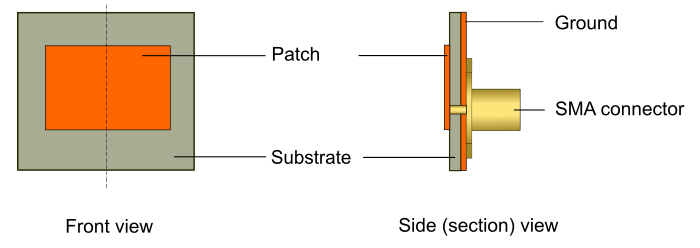
\includegraphics[width=0.8\linewidth]{figs/patch_microstrip_pin_fed.png}
    \caption{Illustration of a microstrip patch antenna on a finite ground using a pin feed (from Altair Community)}\label{fig:patch}
\end{figure}

Procedure antenna:
\begin{enumerate}
    \item Calibrate the NanoVNA (\url{nanovna.com}) to the desired frequency band.
    \item Solder the SMA connector to the patch antenna.
    \item  Connect your antenna to the NanoVNA, using \texttt{CH0}.
    \item Set the VNA to reflect (S11) mode: \texttt{DISPLAY > CHANNEL > CH0 REFLECT}.
    \item Refer to the S-parameter details at \url{www.antenna-theory.com/definitions/sparameters.php}. If clarification is needed, consult your lab assistant.
    \item The antenna is tuned when the S11 curve reaches its minimum at \SI{917}{\mega\hertz}. Aim for an antenna bandwidth of at least \SI{1}{\mega\hertz} (S11 below \SI{-10}{dB} around the target frequency).
\item Plot the S11 curve for your antenna, identify the frequency at which it radiates most effectively, and determine the antenna bandwidth.
\item Carefully trim small sections from the copper corners of the patch antenna to decrease the patch size and adjust the radiating frequency of the antenna. \textbf{Before beginning, seek additional details from your lab instructor on the cutting process. Additionally, exercise caution as sharp tools are involved—cut away from the body (and fingers) and ensure the antenna is placed flat on the table.}
\item Iterate the process of reading S11 and making cuts until the desired target frequency is achieved (steps 7-9).
\item Show your results to the lab assistant before continuing to the next assignment.
\end{enumerate}


\section{Construct your own \gls{usrp} housing}
To not damage the delicate electronics, the B210 should be sealed via a casing. See~\cref{fig:b210-case} for an exploded view of the casing developed by Dramco for the \gls{usrp} B210. 

Sequence of instructions:
\begin{enumerate}
    \item Place the bolts in the holders (11, 21, 22 and 12)
    \item Place the holders on the sides of the casings, in the outer sides of the side (1,2, 3 and 4)
    \item Assemble the top and the sides (1 and 3), not the front (4) or back (2)
    \item Place the B210 inside the casing, aligned with holes of the holders
    \item Complete the assembly by mounting the front and back, encapsulating the B210.
\end{enumerate}

\begin{figure}
    \centering
    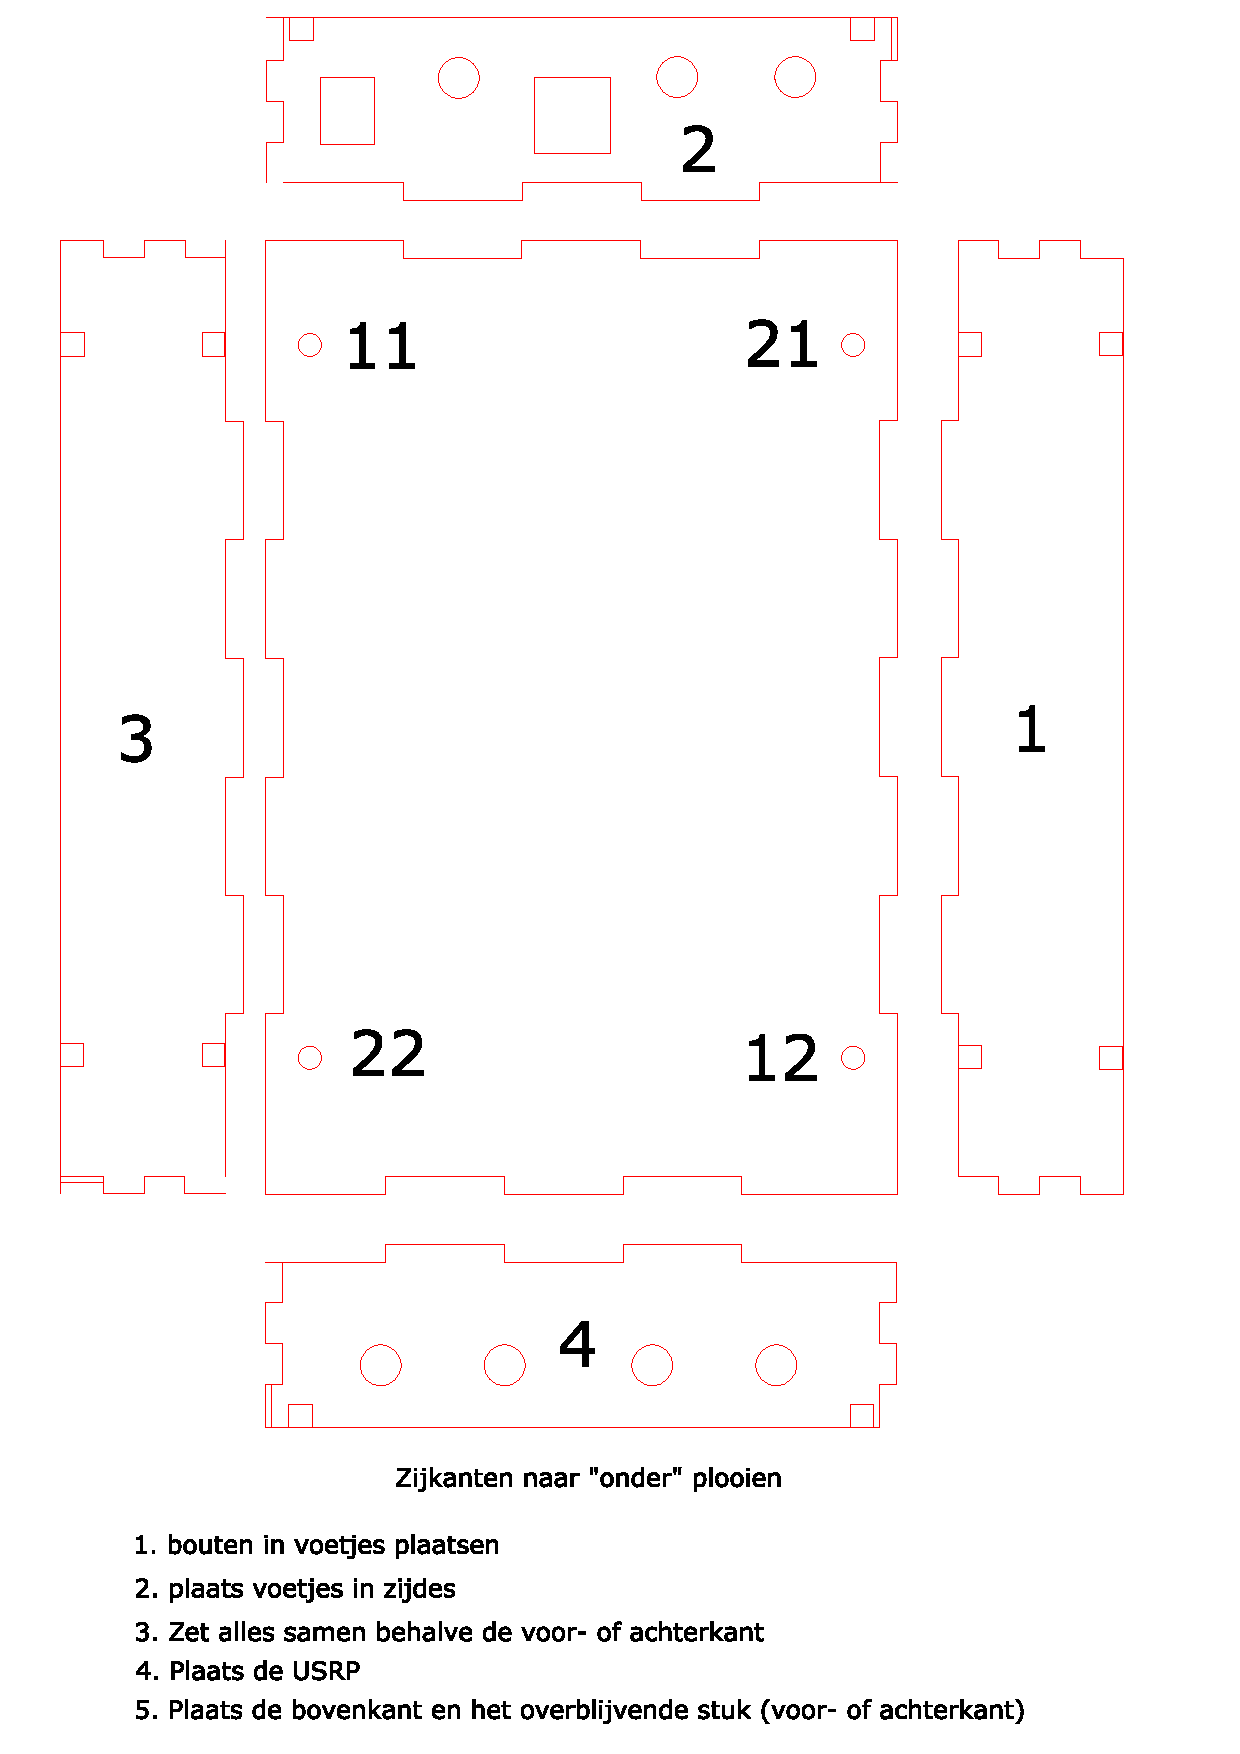
\includegraphics[clip, trim=0mm 50mm 0mm 0mm, width=0.8\textwidth]{figs/assemble_case.pdf}\caption{Exploded view of the B210 casing. The numbers indicates which component should be placed where.}\label{fig:b210-case}
\end{figure}

%\chapter {Scripts Manipulation}

In this lab exercises, you will use the GNU~Radio framework to test and evaluate the performance of an \gls{ofdm} system developed in an \gls{sdr} framework. Some useful Linux commands for easy file manipulation within the terminal window will be given. Afterwards, procedures for starting an \gls{ofdm} transceiver and given GUIs will be explained.

\section{Useful Linux Commands and Hints}
\begin{itemize}
	\item[$\bullet$] \texttt{man {command}} = This opens the help file for the specified command. For example, type man pwd.
	\item[$\bullet$] \texttt{pwd} = Print working directory.
	\item[$\bullet$] \texttt{ls} = List files.
	\item[$\bullet$] \texttt{cd} = Change directory.
	\item[$\bullet$] \texttt{mkdir} = Create a new directory.
	\item[$\bullet$] \texttt{cp} = Copy a file.
	\item[$\bullet$] \texttt{cp -r} = Copy a directory recursively.
	\item[$\bullet$] \texttt{ps -e} = Lists all current running processes
	%\item[$\bullet$] \texttt{su} =Enter root or superuser mode
	\item[$\bullet$] \texttt{grep} = Searches and prints lines matching a given pattern.
	\item[$\bullet$] \texttt{vim} = A shell based text editor.
	\item[$\bullet$] \texttt{killall} = Kills all processes matching a given name or ID number.
	\item[$\bullet$] \texttt{rm} = Removes a file.
	%\item[$\bullet$] \texttt{rm -rf} = Removes a directory.
	\item[$\bullet$] \texttt{chmod} = Change read, write and execute permissions for the owner, group, and guest users.
	%\item[$\bullet$] \texttt{<CTRL>Z} = Suspend process (application).
	\item[$\bullet$] \texttt{<CTRL>C} = Abort process (application).
	\item[$\bullet$] \texttt{./} = Current directory.
	\item[$\bullet$] \texttt{../} = Parent directory of the current directory.
	\item[$\bullet$] \texttt{<TAB>} = Command line completion (automatically fills in partially typed commands).
	\item[$\bullet$] middle mouse button click - paste the previously selected text
	%\item[$\bullet$] \texttt{\ti} = home directory for your login.
	%\item[$\bullet$] \texttt{./} = root directory
\end{itemize}

\section {OFDM System Scripts Manipulation}\label{app:scman}
\begin{enumerate}
	\item In home directory create \textbf{omnilog} directory that will be used for storing the log files required for system configuration
	\item Go to \textbf{omnilog} directory and create the FIFO pipe \textbf{channel} which will be used for communication between transmitter and receiver in \textbf{local environment} mode by executing\newline \texttt{mkfifo channel}
	\item Within the terminal window go to your work directory \newline \texttt{cd /opt/sources/ofdm\_ti\_praktikum/ofdm\_ti\_praktikum/src/apps}
 	\item Make a omniorb configuration file which will be stored in \textbf{\textasciitilde/omnilog/ }by executing\newline \texttt{./mk\_configuration} \textbf{your\_comp}\newline where \textbf{your\_comp} is your PC hostname.
	\item Start the CORBA name and event service by executing the script\newline \texttt{./Setup\_Local\_Environment}\newline \textbf{Note: ignore the warning messages.}
	\item Export environment variables\newline \texttt{. /opt/gnuradio/bin/environment}
	\item In order to set OMNIORB configuration file type\newline export \texttt{OMNIORB\_CONFIG=\textasciitilde/omnilog/omniORB-\textbf{your\_comp}.cfg}\newline \textbf{Note: last two actions need to be repeated in all active terminals.}
	\item To check if name service is correctly running type\newline
	\texttt{nameclt list}\newline
	and the list of initiated name clients should be shown in the terminal window.
	\item Transmitter (Tx) is started by typing\newline 
	\texttt{./usrp\_tx}\newline 
	Prior to actually execute the script, take a look at options that can be configured from command line by typing\newline
	\texttt{./usrp\_tx \option help}\newline
	Here is the list of options:
	\begin{itemize}
 		\item  \texttt{h, \option help}            show this help message and exit
 		\item \texttt{-f FREQ, \option freq=FREQ}  set Tx and/or Rx frequency to FREQ [default=none]
		%\item    \texttt{-d SUBDEV, \option subdev=SUBDEV} select USRP Tx/Rx side A or B
		\item  \texttt{-which-usrp=WHICH\_USRP} select USRP box to use
		%\item   \texttt{-T TX\_SUBDEV\_SPEC, \option tx-subdev-spec=TX\_SUBDEV\_SPEC} select USRP Tx side A or B
		%\item    \texttt{\option measure    }         enable throughput measure, usrp disabled
		\item    \texttt{\option from-file=FROM\_FILE} Sent recorded stream with USRP
		\item    \texttt{\option to-file=TO\_FILE}     Record transmitter to disk, not being sent to USRP
		\item    \texttt{-e INTERFACE, \option interface=INTERFACE} select Ethernet interface, default is eth0
		\item   \texttt{-m MAC\_ADDR, \option mac-addr=MAC\_ADDR} select USRP by MAC address, default is auto-select
		\item    \texttt{\option usrp2}               Use USRP2 Interface
		\item    \texttt{\option fft-length=FFT\_LENGTH} set the number of FFT bins [default=512]
		\item   \texttt{-a AMPL, \option rms-amplitude=AMPL} set total bandwidth. [default=500k]
		\item      \texttt{\option tx-freq=FREQ}     set transmit frequency to FREQ [default=none]
		\item     \texttt{\option snr=SNR}           Simulate AWGN channel
		\item      \texttt{\option freqoff=FREQOFF}   Simulate frequency offset [default=none]
		\item     \texttt{\option samplingoffset=SAMPLINGOFFSET} Simulate sampling frequency offset [default=none]
		\item      \texttt{\option awgn}              Enable static AWGN power for BER measurement
		%\item      \texttt{\option online-work}       Force the ofdm transmitter to work during file record [default=False]
		%\item      \texttt{\option stations=STATIONS} Mobile station count
		\item      \texttt{\option data-blocks=DATA\_BLOCKS} Set the number of data blocks per OFDM frame [default=9]
		\item      \texttt{\option subcarriers=SUBCARRIERS} Set the number of occupied FFT bins. Default: FFT window size - Pilot Subcarriers
		\item      \texttt{\option cp-length=CP\_LENGTH} Set the unique ID number for each node within the system
		\item      \texttt{\option station-id=STATION\_ID} Set IP address or hostname that hosts the CORBA NameService
		\item      \texttt{\option nameservice-ip=NAMESERVICE\_IP}
		\item      \texttt{\option nameservice-port=NAMESERVICE\_PORT} Set access port to NameService
		\item      \texttt{\option log}               enable file logs [default=False]
		\item      \texttt{\option debug}             Enable debugging mode [default=False]
	\end{itemize}

	\item For example, in order to start transmission over USRP, execute the script with following parameters \newline \texttt{./usrp\_tx -f 2.45G \option bandwidth=2M \option fft-length=256 \option subcarriers=200 \newline
	\option station-id=100 \option nameservice-ip=\textbf{your\_comp}}
	\item Similarly, in order to start transmission in local environment in AWGN channel with SNR = 20 dB, execute the script with following parameters 
	\newline \texttt{./usrp\_tx \option to-file channel \option bandwidth=2M \option fft-length=256 \option subcarriers=200\newline 
	\option station-id=100 \option nameservice-ip=\textbf{your\_comp} \option awgn \option berm \option snr=20}.
	\item Receiver (Rx) is started by typing\newline
	\texttt{./usrp\_rx}\newline
	Prior to actually execute the script, take a look at options that can be configured from command line by typing\newline
	\texttt{./usrp\_rx \option help}\newline 
	Here is the list of options:
  \begin{itemize}
 		\item \texttt{h, \option help}            show this help message and exit
 		\item \texttt{-f FREQ, \option freq=FREQ}  set Tx and/or Rx frequency to FREQ [default=none]
		%\item    \texttt{-d SUBDEV, \option subdev=SUBDEV} select USRP Tx/Rx side A or B
		\item  \texttt{\option which-usrp=WHICH\_USRP} select USRP box to use
		%\item   \texttt{-R RX\_SUBDEV\_SPEC, \option rx-subdev-spec=RX\_SUBDEV\_SPEC} select USRP Rx side A or B
		\item  \texttt{\option rx-gain=GAIN}        set receiver gain in dB [default=midpoint].  See also \option show-rx-gain-range
		\item  \texttt{\option show-rx-gain-range}  print min and max Rx gain available on selected daughterboard
  		\item  \texttt{\option from-file=FROM\_FILE} Run Receiver on recorded stream
  		\item  \texttt{\option to-file=TO\_FILE}     Record stream from USRP to disk, no processing
  		\item  \texttt{-e INTERFACE, \option interface=INTERFACE} select Ethernet interface, default is eth0
  		\item  \texttt{-m MAC\_ADDR, \option mac-addr=MAC\_ADDR} select USRP by MAC address, default is auto-select
  		\item  \texttt{\option usrp2}               Use USRP2 Interface
  		\item  \texttt{\option event-rxbaseband }   Enable RX baseband via event channel alps
  		\item  \texttt{\option fft-length=FFT\_LENGTH} set the number of FFT bins [default=512]
  		\item  \texttt{\option disable-ctf-enhancer}  Disable Enhancing the MSE of CTF
  		\item  \texttt{\option scatterplot}         Enable the GUI interface for showing constellation diagrams of the received signal
  		\item  \texttt{\option bandwidth=BANDWIDTH} set total bandwidth. [default=500k]
   		\item  \texttt{\option rx-freq=FREQ}      set receive frequency to FREQ [default=none]
   		\item  \texttt{\option online-work}       Force the OFDM receiver to work during file record [default=False]
   		%\item  \texttt{\option measure}           enable throughput measure
    		\item  \texttt{\option data-blocks=DATA\_BLOCKS} set the number of data blocks per OFDM frame [default=9]
    		\item \texttt{ \option subcarriers=SUBCARRIERS} set the number of occupied FFT bins. Default: FFT window size - Pilot Subcarriers
   		\item \texttt{ \option cp-length=CP\_LENGTH} set the number of bits in the cyclic prefix. Default: 12.5% of fft window size
   		\item  \texttt{\option station-id=STATION\_ID} Set the unique ID number for each node within the system
   		\item  \texttt{\option nameservice-ip=NAMESERVICE\_IP} Set IP address or hostname that hosts the CORBA NameService
   		\item  \texttt{\option nameservice-port=NAMESERVICE\_PORT} Set access port to NameService
   		\item  \texttt{\option log}               Enable file logs [default=False]
		\item  \texttt{\option log-freq-off}	Enable log of frequency offset estimation
   		\item   \texttt{\option debug}             Enable debugging mode [default=False]
   		\item   \texttt{\option disable-freq-sync} Disabling frequency synchronization stage
    		\item  \texttt{\option disable-equalization} Disabling equalization stage
    		\item  \texttt{\option disable-phase-tracking} Disabling phase tracking stage
    		\item  \texttt{\option disable-time-sync} Disabling time synchronization stage
	\end{itemize}

	\item For example, in order to start reception over USRP, execute the script with following parameters \newline \texttt{./usrp\_rx -f 2.45G \option bandwidth=2M \option fft-length=256 \option subcarriers=200 \newline
	\option station-id=1 \option nameservice-ip=\textbf{your\_comp} \option scatterplot}
	\item Similarly, in order to start transmission in local environment in AWGN channel, execute the script with following parameters \newline 
	\texttt{./usrp\_rx \option from-file channel \option bandwidth=2M \option fft-length=256 \option subcarriers=200\newline
	\option station-id=1 \option nameservice-ip=\textbf{your\_comp} \option scatterplot}
	\item Resource manager (that will be implements in  different scripts for different exercises)  is started by executing the script\newline
	\texttt{./run\_script ../python/exercise\_x\_x.py}
% 		\item In order to start system's GUIs do \newline 
% 	\texttt{cd ~/workspace/gnuradio/branches/ofdm\_system\_praktikum/src/qt/gui}
% 	\item Tx's GUI is started by executing\newline
% 	\texttt{./qtgui \option tx \option nameservice=lovas \option port=50001}
% 	\item Rx's GUI is started by executing\newline
% 	\texttt{./qtgui \option rx \option nameservice=lovas \option port=5000}
% 	\item Constellation plots can be observed by going into directory \newline 
% 	\texttt{~/workspace/gnuradio/branches/ofdm\_system\_praktikum/src/qt/scatterplots} 
% 	\newline and executing the script \newline 
% 	\texttt{./scatterplot-gui}
\end{enumerate}


\section {GUI Scripts Manipulation}\label{app:guiman}
\begin{enumerate}
		\item In order to start system's GUIs do \newline 
	\texttt{cd /opt/sources/ofdm\_ti\_praktikum/ofdm\_ti\_praktikum/src/qt/gui}
	\item Tx's GUI is started by executing\newline
	\texttt{./qtgui \option tx \option nameservice=}\textbf{your\_comp}
	\item Rx's GUI is started by executing\newline
	\texttt{./qtgui \option rx \option nameservice=}\textbf{your\_comp}
	\item Constellation plots can be observed by going into directory \newline 
	\texttt{cd /opt/sources/ofdm\_ti\_praktikum/ofdm\_ti\_praktikum/src/qt/scatterplot}
	\newline and executing the script \newline 
	\texttt{./scatterplot-gui}
\end{enumerate}


\chapter{Evaluation}\glsresetall

Evaluation of this lab session will consider students' work attitude throughout the session and a final test to assess their acquisition of requisite skills and knowledge.

Students have the option to collaborate in groups of up to two. However, it's essential to note that assignments must be completed individually. This means each student should be capable of repeating the lab session independently, as their performance will be evaluated during the final test. Additionally, when the students are referred to external sources during the assignment, this must be also known for the final test.
Further instructions will be given during the lab sessions.

Things you need to know (non-exhaustive list):
\begin{itemize}
    \item What is meant by \gls{bb}?
    \item How does the B210 get \gls{iq} samples?
    \item What was the relation between the patch antenna area and the carrier frequency of the antenna?
    \item What does the S11-parameter tell you about your antenna?
    \item How does \textit{pack K bits} block work in \gls{grc}?
    \item What is the \textit{throttle} block, and when do you (not) need it?
    \item What is the difference between streams and vectors in GNU Radio?
    \item How do you calibrate a \gls{vna} and what does each step do?
    \item Which RF architecture is used by the \gls{usrp} B210?
    \item What is frequency selective fading?
    \item How is \gls{isi} mitigated in \gls{ofdm} systems?
    \item What is the relation between a N-\gls{qam} (with N the number of constellation points) and the number of bits per symbol?
    \item What technique is used in \gls{ofdm} to go from a set of parallel symbols to one \gls{ofdm} symbol?  
    \item Why does the \textit{Schmidl \& Cox Synchronization} block does not need to a-priori know the sync word symbols?
    \item What does the plateau detector do in GNU~Radio, and why is this needed?
\end{itemize}




%----------------------------------------------------------------------------------------
%	BIBLIOGRAPHY
%----------------------------------------------------------------------------------------
\clearpage
\printbibliography

%----------------------------------------------------------------------------------------

\end{document}
